\documentclass[a4paper,12pt]{scrreprt}
\usepackage[utf8]{inputenc}
\usepackage[T1]{fontenc}
\usepackage{amsmath}
\usepackage{amssymb}
\usepackage[ngerman]{babel}
\usepackage{enumerate}
\usepackage{array}
%\usepackage{here}
\usepackage{graphicx}
\usepackage{listings}
\newcommand{\Nb}[1]{\textbf{#1}}
\newcommand{\itemd}[1]{\item{\textbf{#1}} }
\usepackage{pgf}
\begin{flushleft}

\end{flushleft}
\usepackage{tikz}
\usetikzlibrary{arrows, automata, positioning, shapes, fit}
\usepackage{enumitem} 
\usepackage{todonotes} 

%opening
\title{Mustererkennung - Schönherr}
\author{Franz Köstner}
\date{WS2013/14}

\begin{document}
\maketitle

\chapter{Zum Begriff ME (pattern recognition)}

\section{Einordnung des Gebietes}

\textbf{Erkennung (Klassifikation) von:}
\begin{itemize}
 \item Bildmustern
 \item Sprachmustern
 \item Zeichenmustern
 \item \dots
\end{itemize}

Muster : Datensatz ( Abstraktion ), zu einer Klasse gehörig\\

\textbf{Unterscheidung von:}
\begin{itemize}
 \item numericher Mustererkennung
 \item Mustererkennung mit KNN
 \item syntaktische Mustererkennung
\end{itemize}

Problem: korrekte Kl.-Einordnung von verschiedenen Formen dereselben Objekte\\
Beispiel: A, $A, \forall$\\
	
Mustererkennung und Bildverarbeitung ist unterschiedlich hat aber vielen Gemeinsamkeiten\\
\begin{itemize}
 \item Bildverarbeitung: Objekte finden
 \item Mustererkennung: Klassifikation von Objekten
\end{itemize}



\begin{figure}[h]
\textbf{Typisches Vorgehen (num. Mustererkennung, KNN)}\\
 \begin{tabular}{>{\centering}p{.5\linewidth} p{7cm} }
    & Beispiel \\
   Rodaten & Pixel-Bild ( evlt. farbig)
    \cr $\downarrow$ & \\
   interessiernde Objekte & Menschen\\
   $\downarrow$& \\
   Merkmalsvekoren &  Nasenlänge , \dots\\
   & \\
   $\downarrow$ f & Funktionen (zu konstruieren), die vom Merkmalsraum in Entscheidungsraum abbilden\\
   Entscheidungsvektoren & \\
   $\downarrow$ & \\
   Klassennzuordnung & \\
 \end{tabular}
\end{figure}

\section{Typische Anwendungen}
  
  \begin{enumerate}[(a)]
   \item Schriftzeichenerkennung \\  $\hookrightarrow$ OCR-Software (optical character recognition)
     \begin{itemize}
   \item Bankbelege: ca. 90\% Erkennung
   \item Erkennen gedruckter Schrift
   \item Handschrift
   \item Unterschriften-Erkennung
  \end{itemize}

  \item Objekterkennung
  \begin{itemize}
   \item Werkstück auf Fließband
   \item Pflanzen zwischen Bahngleisen
  \end{itemize}
  
  \item Qualitätskontrolle
  \begin{itemize}
   \item Produktprüfung: Bsp.: Dachziegel (Risse)
  \end{itemize}
  
  \item Fernerkundung
  \begin{itemize}
   \item Lagerstätten für Ressourcen
   \item Waldbeschaffenheit
   \item Umwelterkennung: Bsp.: Land-Wasser-Grenzen
  \end{itemize}

 \item medizinische Anwendungen
  \begin{itemize}
   \item EKG
   \item EEG
   \item CT-Bilder
   \item Rönten-Bilder
   \item Mikroskop-Bilder
  \end{itemize}

  \item  Auswertung seismographischer Messungen
  \begin{itemize}
   \item Erdbeben?
  \end{itemize}
  
  \item  Roboter-Fußball
  \begin{itemize}
   \item Robotererkennung
   \item Ballerkennung
   \item Spielfelderkennung
   \item Torerkennung
  \end{itemize}
  
  \item Sprachverarbeitung
  \begin{itemize}
   \item Worterkennung
   \item Sprechererkennung
  \end{itemize}
  
  \item Fingerabdruckerkennung
  \item  Gesichtserkennung
  \item Iriserkennung
  \item Handerkennung
  \item CRM-Anwendungen (customer relationship management
 \end{enumerate}
 
 \section{Begriffe und Bezeichnungen}
 
  Muster:\\
 $ \underbrace{\rightarrow}_{informal} $ Datensatz (Komponenten mit Funktionen)\\
  $ \underbrace{\rightarrow}_{formal} $  $f(x) = \begin{pmatrix}{c} f_1(x_1,x_2,\dots,x_n) \\ \dots \\ f_n(x_1,x_2,\dots,x_n) \end{pmatrix} $\\	
\vskip .5cm
\textbf{Muster-Beispiele:}\\
\begin{enumerate}[(a)]
 \item Sprache (mit Mikrofon aufgenommen)\\ $f(t)$ - elektrischer Spannungsverlauf
 \item Schwarzweiß-Bild f(x,y) - Grauwert im Punkt (x,y)
 \item Fernsehbild $f(x,y,t) =  \begin{pmatrix}{c} f_r(x,y,t) \\  f_g(x,y,t) \\  f_b(x,y,t) \\  \end{pmatrix} $
\end{enumerate}

Mustererkennung - Analyse und Klassifikation von Mustern\\

Merkmale: Daten zur Beschreibung eines Objektes\\
\begin{itemize}
 \item Name
 \item Datentyp
 \item Wert
\end{itemize}

n - Anahl (relevanter ) Merkmale\\
\vskip .5cm
Obejk: Menge von Merkmalswerten ( eigentlich Bild eines Objektes)\\
Klasse: Menge von zusammengehörigen Objekten\\
\vskip .5 cm
Stichprobe: endliche Menge von Objekten\\
\begin{itemize}
 \item klassifizierte
 \item unklassifizierte
\end{itemize}
\vskip 1cm
\begin{enumerate}[]
 \item Klassifikator: Alg., der Obj. Klassen zuordnet
 \begin{enumerate}[-]
  \item Güte des Klassifikators: z.B. $\frac{Anzahl korrekter Klassifikationen}{Anzahl aller Klassifikationen }$
 \end{enumerate}
\item Lernen eines Klassifikators ( mit Lehrer)
\begin{enumerate}[-]
 \item   anhand einer klassifizierten Strichprobe ( iterativ)
\end{enumerate}
  \item Clustern ( ohne Lehrer)
  \begin{enumerate}[-]
   \item unüberwachtes ``Lernen``, d.h. aufwendige Konstruktion eines Klassifikators 
  \end{enumerate}
\end{enumerate}

\section{ Merkmale und Invarianten}
Robustheit der Merkmale gegen Störungen ist wünschenswert  
\begin{itemize}
 \item Robustheit gegen geometrische Transformation
 \begin{itemize}
  \item Skalierung
  \item Rotation
  \item Translation
 \end{itemize}
 \item Signalrauschen
 \item Deformationen (Lächeln $\rightarrow$ Gesichtsdeformation )
\end{itemize}
Invarianz geben alle Störungen unmöglich

\subsection{Invarianten}

Merkmale, die bezüglich bestimmten Transformation konstant sind:
\begin{itemize}
 \item Flächeninhalte invariant gegen Translation und Rotation (kann bei Rundungen Fehler erzeugen)
 \item aber nicht gegen Skalierung
\end{itemize}

\textbf{Invariantentheorie:}\\
Welche Merkmale sind gegen welche Transformation invariant?\\
\vskip .2cm
Motivation:\\
Erkennen von gestörten Mustern\\

\textbf{wichtige Transformationen:}
\begin{itemize}
 \item Skalierung: $ y= c \cdot x$ ( c ist Konstante ) 
 \item Translation: $ y = x + a $ ( a ist konstanter Vektor )
 \item Rotation um:
 \begin{itemize}
  \item Winkel $\varphi$
  \begin{itemize}
   \item gegen: UZS: $ y = (\begin{pmatrix}{ c c } 
                            \cos \varphi & -\sin \varphi\\
                            \sin \varphi & \cos \varphi\\
                           \end{pmatrix})$
  \end{itemize}
 \end{itemize}
 \item affine Transformation: y = A x + a ( A: Matrix, a geg. Vektor)
 \item Projektion $y_1 = \frac{a_10 + a_11 x_1 + a_12 x_2}{1 + a_31 x1 + a_32 x_2}$\\
		  $y_2 = \frac{a_20 + a_21 x_1 + a_22 x_2}{1 + a_31 x1 + a_32 x_2}$
\end{itemize}

Affine Invarianten - ein Beispiel\\
$ p_0 , p_1 , p_2 , p $ - 4 Punkte\\
sodass $p_1 - p_0$ und $p_2 - p_0$ linear unabhängig sind\\
dann existieren $\lambda_1,\lambda_2$ , so dass\\
$ p = p_0 + \lambda_1 (p_1 - p_0) + \lambda_2 (p_2 - p_0) $ \\

\begin{figure}[h]
 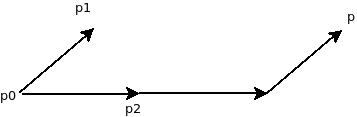
\includegraphics[width=7cm]{./abbildungen/linunab.jpeg}
 \caption{Beispiel: $p=0.5(p_1-p_0)+2(p_2-p_0)$}
\end{figure}

$Ap+a = Ap_0 + a+ \lambda_1(A_1 + a - A_0 - a)+ \lambda_2(A_2 + a - A_0 - a)$
$\hookrightarrow \lambda_1 , \lambda_2$ invariant gegen affine Transformationen

\underline{Wichtig}: Entsprechung der Basispunkte\\
$p - q $ $ p_1 - q_1 \dots $
zu garantieren (per Augenmaß)\\
Diese Aufgabe ist ein Referenzproblem\\

Danach $A,a$ bestimmbar\\

Eigenschaft affiner Transformationen:\\
\begin{itemize}
 \item Geraden gehen in Geraden über. (Collinearität)
 \item Abstände von Punkte ändern sich um einen gemeinsamen Faktor. Bei Projektiven Transformationen gibt es keinen gemeinsamen Faktor. Projektive Transformationen sind auch collinear.
 
\end{itemize}

Das Doppelverhältnis:\\
Situationsbeschreibung\\
4 collineare Punkte in einem Referenzmuster gegeben $(x_i)$\\
4 Bildpunkte (nach proj. Abbildung) gegeben $(y_i)$\\
Annahme: Referenzproblem gelöst\\

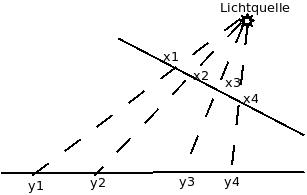
\includegraphics[width=7cm]{./abbildungen/Doppelverhaeltnis.jpeg}

Doppelverhältnis:
$DV(x) = \frac{\frac{x_1 - x_2}{ x_1 - x_3}} {\frac{x_4 - x_2 }{x4_-x_3}} $

\textbf{Satz}: DV(x) = DV(y), d.h. Invarianz gegen proj. Transformation\\

\textbf{Übung:}
Aufgabe1:\\
Aufnahmen von zwei projektiven Kameras. Es existieren in Bild 1 4 Charakteristische Punkte.
 \begin{itemize}
  \item $P_1 = (0,1)$
  \item $P_2 = (3,10)$
  \item $P_3 = (4,13)$
  \item $P_4 = (6,19)$
 \end{itemize}
Das zweite Bild enthält eine möglicherweise entsprechende Strecke.
\begin{itemize}
 \item $Q_1=(-13,26)$
 \item $Q_2 = (-\frac{13}{7}, \frac{26}{7} ) $
 \item $Q_2 = (-\frac{13}{9}, \frac{26}{9} ) $
 \item $Q_2 = ( -1, 2 ) $
\end{itemize}

Doppelverhältnis von q = 0.5\\
Doppelverhältnis von p = 0.5\\

Aufgabe2:\\
 \begin{itemize}
  \item $P_1 = (0,3)$
  \item $P_2 = (1,2)$
  \item $P_3 = (2,1)$
  \item $P_4 = (3,0)$
 \end{itemize}
 Das zweite Bild enthält eine Möglicherweise entsprechende Strecke mit den mutmaßlich entsprechenden Punkten $ q_1 $ bis $ q_3 $. \\
 \begin{itemize}
 \item $Q_1 = (0,6)$
 \item $Q_2 = (2,4)$
 \item $Q_2 = (4,2)$ 
 \end{itemize}
 Wo müsste ein vierter Referenzpunkt gefunden werden?
 Lösung: $q_4 = (0,6)$\\
 
\subsection{Flächeninvarianten}
 
 \begin{enumerate}[(a)]
  \item Determinantenmethode
  \begin{description}
   \item Berechnnung von Streckenlängen, Dreiecksflächen, Tetraedervolumina, \dots können mittels der Eckpunkt mithilfe von Determinanten berechnet werden.
 Untersuchung des Verhaltens von Determinanten bei Transformationen $\rightarrow$ mögliche eine Reihe von Determinaten abzuleiten
  \end{description}
  \item Formfaktor F
  \begin{description}
   \item $ F = \frac {u^2}{4f} $
   \item u - Umfang
   \item f - Fläche
   \item Beispiel: Kreis mit Durchmesser 1
   \item F(Kreis) = $\frac{ (\pi * d)^2 }{4 +*\frac{\pi}{4} d^2} = \pi $
   \item F(Quadrat) = $ \frac{ (4 * a)^2 }{ 4 * a^2} = 4  $
   \item F beschreibt die Unrundheit einer Fläche
   \item Im Allgemeinen ist kein Rückschluss auf die Form möglich.
  \end{description}
 \end{enumerate}

 \subsection{Momente}
 
 Berechnung von geometrischer Momente:\\
 F sei eine Fläche (z.B. Kreis)\\
 Momente der Ordnung p + q\\
 $$ M_{pq} =  \iint_F  x^p * y^q dx dy $$ \\
 Interpretation von Momenten\\
 $M_{00} = $ Fläche von F\\
 $M_{10}/M_{00} = $ X-Koordinate des Schwerpunktes\\
 $M_{01}/M_{00} = $ Y-Koordinate des Schwerpunktes\\
 $M_{20},M_{02} = $ Trägheitsmomente bezüglich Koordinaten-Achsen\\
 $M_{20}+M_{02} = $ polares Trägheitsmoment bezüglich (0,0)\\
 $M_{11} = $ ? \\
 
 gegeben: flächenhaftes Objekt\\
 Berechnung des Schwerpunktes\\
 Translation der Fläche, so dass Schwerpunkt auf  (0,0) liegt.\\
 $ \hookrightarrow$ Fläche F
 
 \subsection{Die Trägheitsellipse}
 
 \textbf{Definition}: Die Ellipse\\
 $$M_{20} * x^2 + 2 * M_{11} * x  * y + M_{02} * y^2 = 1$$
  heißt Trägheitsellipse in Mittelpunktelage einer Fläche F.\\
  Bemerkung: Es gilt immer $ M_{20} * M_{02} \ge M_{11}^2 $, so dass es sich wirklich um einne Ellipse handelt.\\
  
  \paragraph{Definition:} Neigung von F gegen X-Achse = Neigung der Trägheitsellipse von F gegen X-Achse\\
  \textbf{Zielstellung:} Feststelllen des Neigungswinkels von F\\
  \\
  F samt Ellipse wird entegen dem Uhrzeitgersinn um den Winkel $\varphi$ gedreht. ( um Koordinatenursprung )\\
  $\hookrightarrow$ neues (u,v)-Koordinatensystem \\
  Im neuen System soll die Ellipse in Hauptachsenlage liegen, dass heißt $\varphi$ ist passend zu wählen.
  
  %\includegraphics[scale=1]{./abbildungen/Trägheitsellipse.jpg}
  
  Berechnung der neuen Momente 2. Ordnung (nach Drehung):\\
  \\
  $M_{20}(\varphi) = \iint_{F'} v^2 dv du$ (F' : F im (u,v)-System)\\
  $ =  \iint_F (x + \cos(\varphi) - y - \sin(\varphi)^2 dx dy $\\
  $ =  \iint_F (x^2 + \cos^2(\varphi) -2*x*y * \sin(\varphi)*\cos(\varphi) + y^2 * sin^2(\varphi)) dx dy $\\
  $ = M_{20} + cos^2(\varphi) - 2 * M_{11} *\sin(\varphi)*\cos(\varphi) + M_{02}*\sin(\varphi)$\\
  Ebenso ergibt sich\
  $ M_02(\varphi) =  M_{02} + cos^2(\varphi) + 2 * M_{11} *\sin(\varphi)*\cos(\varphi) + M_{20}*\sin(\varphi)$\\
  Ferner gilt:\\
  $M_{11}(\varphi) = \iint u * v du dv$\\
  $ = \iint_F ( x *\cos(\varphi) - y * \sin(\varphi) ) *  ( x *\sin(\varphi) + y * \cos(\varphi) ) dx dy $\\
  $ = \iint_F ( x^2 * \sin(\varphi) * \cos(\varphi) ) dxdy \iint_F ( x*y * \cos^2(\varphi) ) dxdy   \iint_F ( x*y*sin^2(\varphi) ) dxdy - \iint_F ( y^2 * \sin(\varphi) * \cos(\varphi) ) dxdy   $\\\
  $ = (M_{20}-M_{02}) * \sin(\varphi) * \cos(\varphi) + M_{11} * (\cos^2(\varphi)-\sin^2(\varphi))$\\
  Nullsetzten dieses Ausdrucks ( also $M_{11} ( \varphi )$ ), wenn Hauptachsenlage der Trägheitsellipse im (u,v)-System zu erreichen.\\
  Division durch $\cos^2(\varphi) ( \varphi \neq \frac{\pi}{2} ) \rightarrow $ Übergang zum Tangens\\
  $\hookrightarrow 0 = (M_{20}-M_{02} * \tan (\varphi) + M_{11} * (1-\tan^2 (\varphi))$\\ 
  Dividieren durch $ M_{20} - M_{02}$ und durch $ (1-\tan^2 (\varphi)) $ und * 2\\
  $\frac{2*M_{11}}{M_{02}-M_{20}} = \frac{2*\tan (\varphi)}{1-\tan^2 (\varphi)} = \tan ( 2 * \varphi ) | (\varphi \neq \frac{\pi}{4}) $\\
  $\hookrightarrow q = \frac{1}{2} * \arctan ( \frac{2 * M_{11}}{M_{02} - M_{20}} ) $\\
  Die Berechnung ist nicht möglich bei Gleichheit von $M_{20}$ und $M_{02} $ Gründe dafür sind mögliche Regelmäßigkeiten der Fläche - Beispiele sindregelmäßige Polygone oder ein Rechteck, welches von der Normalelage um $45^\circ$ gedreht ist. \\
  Bemerkung: Wenn eine Fläche gedreht wird, dreht sich die zugehörige Trägheitsellipse automatisch mit.\\
  \\
  Ellipsengleichung im Hauptachsenlage (allgemein)
  \\
  $\frac{u^2}{a^2} + \frac{v^2}{b^2} = 1 $\\
  \\
  a - Länge vom (0,0) bis zum linken/rechten Scheitelpunkt\\
  b - Länge vom (0,0) bis zum unteren/oberen Scheitelpunkt\\
  \\
  Setze (passend gewählt):\\
  $a = \frac{1}{\sqrt{M_{20}(\varphi)}}$
  $b = \frac{1}{\sqrt{M_{02}(\varphi)}}$\\
  $\downarrow$\\
  $M_{20}(\varphi) v^2 + M_{02} (\varphi) v^2 = 1$\\
  \\
  Ausblick:
  \begin{enumerate}[(a)]
   \item Übertragung zur komplexen Ebene (x + iy) - Berechnung komplexer Momente\\
	  Bekannt: $H_v$-Invarianten ($H_1,\dots,H_{12}$)
   \item Berechnung von Linienmomenten mit Kurvenintegralen
  \end{enumerate}

  \chapter{Mustervergleich (Matching) }
  
  \section{Abstandsmaße}
  
  \textbf{Referenzmuster} (template) sei gegeben - mit mathemtischem Modell\\
  beziehungweise für jede Klasse ein Referenzmuster $\rightarrow$ modellbasiertes Matching\\
  Problem: neues Muster ähnlich zu einem Referenzmuster?\\
  Berücksichtigung von:
  \begin{itemize}
   \item Position
   \item Skalierung
   \item evtl. Rotation
   \item Orientierung
  \end{itemize}
  Muster durch Signalwerte gegeben:\\
  Beispiel: Grauwerte im interessiernden Gebiet G\\
  r(x,y) - Grauwerte der Referenzmusters, $(x,y) \in G$\\
  f(x,y) - Grauwerte eines gegeben Bildes\\
  Abstand zwischen 2 Bildern ( Bsp )\\
  \begin{enumerate}[]
   \item $a_1$= max | f(x,y)- r(x,y) | , $(x,y) \in G$
   \item $ a_2 =  \iint_G ( f(x,y) - r (x,y) )^2 dx dy $\\
   \item $ a_3 = \sum_{(x,y) \in G} ( f(x,y) - r (x,y) )^2 dx dy $\\
  \end{enumerate}
Fall qualitative Merkmale: Hamming-Distanz\\
$a_4 = \sum_i | x_i - y_i | $\\
    
    \subsection{Abstand endlicher Punktmengen}
    
    Nutzung für:
\begin{itemize}
 \item Obejekterkennung in Bildern
 \item Handschrifterkennung
\end{itemize}

$A, B$ \dots endliche Punktmengen\\
Abstand zweier Punkte:\\ $d(a,b)=\|a-b\|$, mit $\|x\|$ gleich Norm von x

Abstand eines Punktes $a$ von Punktmenge $B$:\\ $d(a,B)=\min\limits_{b\in B}
\|a-b\|$
BILD1\\
Abstand zweier Punktmengen:\\
$n(A)$ = Anzahl der Elemente in $A$\\
$n(B)$ = Anzahl der Elemente in $B$\\
$d_1(A,B)=\min\limits_{a\in A} d(a,B)$\\
BILD2\\
$d_1(A,B)=0$ bei Gleichheit zweier Punkte $a,b$\\
$d_2(A,B)=\max\limits_{a\in A} d(a,B)$\\
$d_3(A,B)=\frac{1}{n(A)}\sum\limits_{a\in A} d(a,B)$, mit $n(X)$ gleich
Anzahl der Punkte in $X$\\

\paragraph{Ungerichtete Abstandsmaße:}
Irgendein Abstandsmaß $d(A,B)$ sei gegeben. \\
$$u_1=min\{d(A,B), d(B,A\}$$
$$u_2=max\{d(A,B), d(B,A\}$$
$$u_3=\frac{d(A,B)+d(B,A)}{2}$$
$$u_4=\frac{n(A)\cdot d(A,B)+n(B)\cdot d(B,A)}{n(A)+n(B)}$$

Wichtig: Robustheit gegenüber Störungen!\\
Hausdorff"=Metrik ($d_2$ mit $u_2$) eher ungeeignet wegen $\max$\\
Kombination von $d_3$ mit$u_2$ ist günstig: $$ u(A,B)=max\left\{
	\frac{1}{n(A)}\sum\limits_{a\in A} d(a,B),
	\frac{1}{n(B)}\sum\limits_{b\in B}d(b,A)\right\}$$
\subsection{Korrelationsmaße als Matching"=Maße}
$x,y$ \ldots Muster"=Vektoren zum Beispiel Pixel"=Grauwerte
$$m=\frac{\langle x,y\rangle}{\|x\|\cdot\|y\|}\text{, dann} -1\le m \le1 \text{ und } x=y\to m=1$$
Falls $y=k\cdot x$, gilt: $m$ ist invariant gegen $k$ ($k\not=0$)
($k$ ist Konstante für den Kontrastunterschied)

$y=x+h$ mit $h$ gleich Vektor mit identischen Komponenten\\
Bilder werden (bei großen $h$"=Werten) als verschieden
bewertet.\\
m sollte invaraint sein gegen Kontrast- und Helligkeitsänderung.\\

\paragraph{Neudefinition des Matching"=Maßes:}%Nb
$ x' $ ist der Vektor mit Durchschnittshelligkeit von $x$ als Komponenten\\
$y'$ ist der Vektor mit Durchschnittshelligkeit von $y$ als
Komponenten

Ersetzen von $x$ durch $x-x'$ und $y$ durch $y-y'$ in der $m$"=Formel. 
Dadurch ergibt sich die zyklische Kreuzkorrelation $m'$:
$$ m'=\frac{\langle x-x', y-y'\rangle}{\|x-x'\|\cdot\|y-y'\|}$$
\paragraph{Prüfung mit 2 pixelbilder: objekt in der hauptdiagonale gleich?
helligkeitsverschiebung? m' benützen. Antwort: sind unterschiedliche
Objekte, bzw. man kann davon ausgehen das es die selben Objekte sein
könnten}

\section{Normalisierung zweier endlicher Punktmengen} Problem: 2
Mengen $A(x,y), B(u,v)$ die möglicherweise dasselbe Objekt darstellen.
$u=f_1(x,y)$ und $v=f_2(x,y)$ (eine Menge Bild der anderen)\\
$f=\begin{pmatrix}f_1\\f_2\end{pmatrix}$ ist damit eine unbekannte
Koordinatentransformation.
\subsection{Berechnung von MSE (mean square error)}
$$MSE=\sum\limits_iw_i\cdot\left[\left( u_i-f_1(x_i,y_i) \right)^2 +
\left( v_i-f_2(x_i,y_i) \right)^2 \right] \rightarrow \text{min} $$ 
mit $w_i$ gleich gegebene Gewichte, der Bedeutung der Punkte
entsprechend zu wählen.\\
Zum Beispiel: $w_i\ge0 \land \sum\limits_iw_i=1$\\
oder: $\underbrace{\forall i: w_i=1}_{\text{bei Gleichwertigkeit}}$\\
\\
Variabel sind dabei die Parameter von $f$. (stehen nicht mit in der Formel)\\
Voraussetzung: $A, B$ haben gleiche Kardinalität.\\
Zuordnung $(u_i, v_i)\leftrightarrow(x_i,y_i)$ müssen bekannt sein,
das heißt alle Referenz"=Probleme gelöst. Die Voraussetzung ist damit
praktisch nie erfüllt.
  
\subsection{Heuristisches Verfahren zur näherungsweisen Lösung für
$MSE\to\min$ für beliebige Punktmengen und ohne bekannte
Referenzbeziehungen:} 

\begin{enumerate}
\setcounter{enumi}{-1}
\item $A$ wird mittels $f^{(0)}=\begin{pmatrix}f_1^{(0)}\\f_2^{(0)}\end{pmatrix}$ so transformiert, dass danach
		$A$ mit $B$ ``grob'' deckungsgleich ist. $f^{(0)}(A)\approx B$
\item Für alle $a\in A$ wird ein $b\in B$ bestimmt mit Abstand
	$d(a,B)$. Sammeln dieser Pseudo"=Referenz Paare in einer Liste $L$
\item Für alle $b\in B$ wird ein $a\in A$ bestimmt mit Abstand
	$d(b,A)$. Sammeln dieser Pseudo"=Referenz Paare in einer Liste $L$
\item $i=i+1$\\
Berechnung einer Transformation $f^{(i)}$ durch Minimierung von MSE in Bezug auf die Pseudo"=Ref"=Paare \item $A=f^{(i)}(A)$
\item Gütekontrolle $d(A,B)$ genügend klein? \\ Falls ja, Stop mit
	Erfolg\\ Falls nein,  goto 1\\ Falls $d(A,B)$ nach zahlreichen Interationen zu groß, dann STOP ohne Erfolg
\end{enumerate}

\section{Die Hough"=Transformation} Detektion von geraden Linien in
einem Bild (meist Konturlinien)\\ Gegebenfalls Vorverarbeitung:
Konturen filtern (mit Sobel"=Filter, Canny"=Filter)\\ Grundlage:
Hesse'sche Normalform der Normalengleichung.\\ \Nb{Übliche
Geradengleichung:} $a*x+b*y+c=0$ (Wenn $b=0\to$ Gleichung nicht
auflösbar nach $y \rightarrow$ parallel zu $y$)\\ $l$ ist die Länge des Lotes von $(0,0)$ zur
Geraden, mit $(0,0)\not\in$ Gerade.\\ $\varphi$ ist der Winkel des
Lotes zur $x$"=Achse.\\ $l=x*\cos{\varphi}+y*\sin{\varphi}$\\ Bild der
Geraden im $(l,\varphi)$"=Koordinatensystem (Hough-Raum) ist ein Punkt, denn  $l$
und $\varphi$ determinieren die Gerade.\\
Beispiel:\\
$y_1 : 2* x -y -3 = 0$\\
$y_2 : y-2= 0$\\
Bild3\\
\subsection{Praktisches Vorgehen (zur Liniendetektion)}
Diskretisierung des Hough"=Raumes $\rightarrow$ rechteckiges
Punktefeld\\
Zuordnung einer Zählvariablen zu jeden solchen Punkt (anfangs 0).\\
Bemerkung: Jedem Pixel im H"=Raum entspricht eine Gerade im
$(x,y)$"=Raum

Berechnung aller Geradenstücke aus Vordergrundpixel im Urbild.
Erhöhung der jeweiligen Zählervariablen im H-Raum zu jedem
Geradenstück. Danach werden die Zählvariablen mit höchsten Werten
ermittelt. Denen entsprechen die wichtigsten Strecken im Urbild. 
Literatur: Haberäcker\\
Erweiterung möglich auf Kreise, Ellipsen, \dots\\


\section{Matching"=Möglichkeiten}
\subsection{Signalorientiertes Matching} 
Bezeichnug für die bisher beschrieben Vorgehensweißen
Grund: direktes Matchen gemessener Signalwerte (Grauwerte von Pixeln)

\subsection{Merkmalsorientiertes Matching}
Matchen auf Grund von Signalwerten abgeleiteter Werte (z.B.: Merkmale, Hough-Koordinaten, \dots)\\
siehe Kapitel \ref{NumerischeKlassifikation}\\

\subsection{Stereo"=Matching}
Aufgabe: Erkennung von 3D"=Objekten aus verschiedenen 2D"=Bildern\\
Problem: Referenz"=Problem lösen bei projektiver Verzerrung
Erkennungsalgorithmus verwenden\\

\subsection{Graph"=Matching} Modellierung komplexer Szenen als
Graphen.\\ Erkennung von Teil"=Szenen:\begin{itemize}
	\item Kommt ein Graph in einem anderen vor?
	\item Sind 2 Graphen gleich?
	\end{itemize}

\chapter{Numerische Klassifikation}
\label{NumerischeKlassifikation}
\section{Aufgabenstellung}
$E^n$ wird betrachtet, heißt Merkmalsraum (n-dim Euklidischer Raum)\\
Objekt $O$: Repräsentation als $n$"=dimensionaler Messwerte"=Vektor\\
$m$"=Anzahl der Klassen\\
$K_i$:  $i$"=te Klasse\\

\Nb{Gesucht:} Zerlegung von $E^n$ in $m$ Gebiete $G_i$, so dass
$$E^n=\bigcup\limits_{i=1}^{m} G_i $$ \\
$$ \forall i \forall j i\not=j \rightarrow G_i\bigcap G_j=\emptyset $$\\
Klassifikator ordnet einem Objekt $O$ $K_i$ zu, falls $x\in G_i$, mit
$x$ Bild von $O$
Problem: Zerlegung soll möglichst gut sein:
\begin{itemize}
 \item entsprechnd der Bedeutung der Klasse
 \item möglichst weniger Echtklassifikationen
\end{itemize}
Ggf. (m+1)-tes Gebiet als Rückweisegebiet vorsehen. 

\subsection{Geometrische Modelle}
Die $G_i$ (Modell) werden mit Musterklassen (Realität) identifiziert. $O\in K_i
\Leftrightarrow x\in G_i$
\subsection{Stochastische Modelle}
Klassifiziert wird nach $x\in G_i$, was nicht $O\in K_i$ bedeuten
muss!

Ursache: Kriterien, die der Klassifikator nicht ``kennt''. (unvollständige Modellierung)

Bsp.: Menschen in Erkältete und Nichterkältete einteilen
Klass."=Kriterien:  husten oder niesen = true
\section{Geometrische Klassifikationsmodelle}
\subsection{Trennfunktionen}
Mehrere Punktmengen in $E^n$ gegeben

\Nb{Definition:} $P1$, $P2\subset E_n$ heißt linear separierbar, falls es eine Hyperebene\\
$$a^\top x+b=0$$\\
gibt, so dass 
$$a^\top x+b>0 \text{, für }x\in P_1$$\\
und\\ $$a^\top x+b<0, \text{ für } x\in P_2$$.\\
\\
Bei 3 separierbaren Klassen in $E^2$ sind 3 Geraden zur Klassifikation
erforderlich. Allgemein: $m$"=Klassen in $E^n$ dann\\
$$\frac{m(m-1)}{2}$$
Trenn-Hyperebenen zu konstruieren.\\
Lineare ist Separierbarkeit nicht offensichtlich.

\subsection{Diskriminanzfunktionen}
Generelle Idee: Konstruktion einer Menge von Funktionen ($m$
Funktionen) $d_i$.\\ $x$ gehört zu $K_i$, wenn $d_i(x)>d_j(x)$, für
$i\not=j$\\
\Nb{Definition:} $E^n$ vollständig in $m$ Gebiete $G_i$ zerlegt.\\
$m$ auf $E^n$ stetige Funktionen $d_i(x)$ heißen
Diskriminanzfunktionen, wenn für alle Nicht"=Randpunkte gilt:\\
$$\forall k \forall j \left[ x\in G_k \land k\not=j \to
	d_k(x)>d_j(x) \right]$$
Trennfunktion zweier Gebiete $G_i, G_j$ ist spezifisch durch die Gleichung:
$$d_i(x) = d_j(x)$$
Lösung des Klassifikations"=Problem durch Berechnung des
\Nb{Klassen"=Index} nach $$k=\text{index}\left\{\max\limits_i{d_i(x)}  \right\}$$


\subsubsection{Konstruktion spezieller Diskriminanzfunktionen}
\begin{enumerate}
	\itemd{Minimum"=Distanz-Klassifikator}\\
	Idee: Beschreibung der Klassen durch
		Referenzmuster (oder Zentren) $z_i$.\\
	Klassifikation: $x$ wird Klasse $K_i$ zugeordnet, wenn der Abstand von
	$x$ zu $z_i$ minimal ist.\\
	Euklidischer Absand $a(x,z_i)$ zwischen $x$ und $z_i$\\
	$$a_1^2 (x,z_i) = || x - z_i ||^2 = x^Tx - 2 z_i^T x + z_i^Tz_i$$\\
	Bemerkung: $a$ oder $a^2$ ist gleichgültig wegen Monotonie von ($|^2$). Die Konstante (bezüglich i) $x^Tx$ auch irrelevant.\\
	Diskriminanzfunktion: $d_i(x)=z_i^\top z_i-2z_i^\top x$\\
	$Klassenindex_i$ linear bezüglich $x$
	 $$k = index \{ \min\limits_{1 \leq i \leq m } d_i(x) \} $$
	
	Trennfläche zwischen 2 Klassen $K_i$ und $K_j$ $d_i(x) = d_j(x) \rightarrow $ vollständige Zerlegung des $E^n$ 
	
	\itemd{NN"=Klassifikator (nächster Nachbar)} Im allgemeinen eine zu ungenaue
		Beschreibung einer Klasse durch nur ein Zentrum $z_i$ $\rightarrow$
		Idee: mehrere Referenzmuster pro Klasse.\\
		$K_i$: Zentren $z_i(j)$ $1\le j\le J(i)$ mit $J$ Anzahl der
		Zentren für $K_i$.\\
		Diskriminanzfunktion (stückweise linear):\\ $$d_i(x)=\min\limits_{1\le j \le J(i)}\left\{ z_i(j)^\top\cdot z_i(j) -2\cdot z_i(j)^\top\cdot x \right\}$$
		$k = index \{ \min\limits_{i} di(x) \}$
	\itemd{KNN"=Klassifikator}\\ Verbesserung des NN"=Klassifikators, indem Ausreißer schwächer berücksichtigt werden.\\
	x sei gegeben und zu klassifizieren\\
	Idee: Berechnung aller 
	$$d_{ij}(x)=z_i(j)^\top\cdot z_i(j) -2\cdot z_i(j)^\top\cdot x$$
	, d.h.$\sum_i d(i)$ Werte
	\begin{itemize}
	 \item i - Klassenindex
	 \item j - Zentrenindex in $K_i$
	\end{itemize}
	Auswahl der $k$ kleinsten $d_{ij}(x)$ (k gegeben).\\
	Klassifikationsregel: Zuordnung von $x$ zu $K_i$, wenn für $i=|$ die meisten $d_{ij}(x)$ unter den k kleinsten vorkommen.\\
	Nichteindeutigkeit ist möglich.\\
	Entscheidung z.B. nach minimaler Summe der entsprechenden $d_{ij}$. Eventuell besser: \dots der entsprechenden Abstände\\
	\\
	Festlegung von k:\\
	k groß $\rightarrow$ schwächerer Einfluss von Ausreißern\\
	$k = 1 \rightarrow$ NN"=Klassifikator

\itemd{Andere Diskriminanzfunktionen}\\
\begin{itemize}
 \item $d(x)=c^T f(x)$ mit $f(x)$ fest vorgegeben
 \item Polynome $\rightarrow$ Polynom-Klassifikator
\end{itemize}
\itemd{Klassifikation mit Rückweisegebiet}\\
Zentren $z_i$ festlegen\\
Festlegung von -Hyperquadern , -kugeln, -ellipsen um die $z_i$ herum.\\
x zu Klassifizieren, $z_7$ am nächsten aber nicht im $Hyperquader_7 \rightarrow$ Rückweisung 
\end{enumerate}

\subsection{Baumklassifikator}
Idee:

\begin{itemize}
 \item Konstruktion achsenparalleler Hyperquader (möglicherweise
Vereinigungen zugelassen)
\item Beschreibung des $i$"=ten Quaders ($1\le i\le m$) durch dessen
Extremalpunkte: $p\left[ i \right]$ und $q\left[ i \right]$
\item Klassifikator: $x\in K_i\leftrightarrow p_j\left[ i \right]\le x_j\le
q_j\left[ i \right]$ mit $i$"=Klassen"= und $j$"=Komponenten"=Index
\item Bestimmung von $p\left[ i \right]$ und $q\left[ i \right]$:\\
$x_1,\dots,x_s$ ist eine vorklassifizierte Punktmenge\\
\begin{large}
$$p_j\left[ i \right]= \min\limits_{r: x\left[r \right]\in
K_i}\left\{ x_j\left[ r\right] \right\}, 
q_j\left[ i \right]= \max\limits_{r: x\left[r \right]\in
K_i}\left\{ x_j\left[ r\right] \right\}$$ 
\end{large}
\end{itemize}
Problem: 
\begin{itemize}
  \item empfindlich gegen Ausreißer in der Punktemenge wegen $\min$ und $\max$
  \item Bestimmung aller $p_j$ und $q_j$ nicht immer erforderlich
\end{itemize}
Problem - Überlappung von Quadern:
\begin{itemize}
  \item Zurückweisung bei $x \in $ Überlappungsgebiet
  \item Zuweisung zu genau einer Klassse (Zusatz-Regeln erfinden)
  \item Zuweisung zu mehreren Klassen
\end{itemize}


\section{Stochastische Klassifizierungs"=Modelle}
\subsection{Problemstellung}
$m$ oder $m+1$ Gebiete des $E^n$ (gegebenenfalls ein
Rückweisungsgebiet)\\
Vollständige Zerlegung des $E^n$ ist gesucht, dabei soll es $m$ echte
Klassen geben.
\begin{description}
  \item{$X$}"= n Komponenten zur Beschreibung eines zufälligen Objekts
  \item{$Y$}"=Zufallsgröße: Bedeutung $Y=i\leftrightarrow$ zufälliges
Objekt $X\in K_i$
  \item{$f(x)$}"= Dichte (stetig) von $X$, wobei x n-dimensionaler Vektor\\
  Ableitung von $P(X \leq x)$ -  einmal pro Komponente von x
  \item{$f(x|y=i)$}"= bedingte Dichte von $X$ unter der Bedingung, dass
$y = i$. Das heißt Ableitung(nach jeder der Komponenten von x) von $P(X \leq x | Y = i)$
\item Bemerkung: Stetigkeit von $f(x)  \rightarrow$ Vorraussetzungen des Satzes von Schwarz 
\end{description}
Von Interesse ist die Beziehung zwischen $f(x)$ und $f(x|Y=i)$.
Nach Satz von der totalen Wahrscheinlichkeit gilt:\\
$$P(X\in(x,x+h{]}=\sum\limits^m_{i=1}P(X\in(x, x+h{]} |Y=i)\cdot
P(Y=i)$$
linke Seite:\\
$$P(X\in(x,x+h{]}=\int\limits^{x_1+h_1}_{x_1}\dots\int\limits^{x_n+h_n}_{x_n}
f(y_1,\dots,y_n)dy_n\dots dy_1$$
Division durch alle $h_i$ und $h_i \rightarrow 0$\\
\begin{large}
$$ \hookrightarrow f(x) = \frac{\partial''P(X_1 \leq x1 , \dots , X_n \leq x_n)}{\partial x_1 , \dots , \partial x_n}$$
\end{large}
rechte Seite:\\
$$ P( x \in (x,x+h| Y= i] \text{ wird analog behandelt}$$
Ergebnis: $$ f(x) | Y=i) $$\\
Also:
$$f(x)=\sum\limits_{i=1}^m f(x|Y=i)+P(Y=i)$$
Ferner von Interesse: $$P(Y=i| X=x)$$ d.h. Wahrscheinlichkeit für 
$\left\{ \text{Objekt}\in K_i \right\}$, wenn Vektor $x$ beobachtet
wurde.\\
Ausgangspunkt: $$P(Y=i \land X\in(x,x+h{]})$$
Umformung auf 2 verschiedene Arten:
\begin{itemize}
 \item einmal 1. Ereignis
 \item einmal 2. Ereignis 
\end{itemize}
in Bedingung schreiben\\
$$P(Y=i|X\in(x, x+h{]})*P(X\in(x, x+h{]})$$
$$=P(X\in(x, x+h{]}|Y=i)*P(Y=i)$$
Dann Division von $P(X\in(x, x+h{]})$ , sowie das Prod.
$h_1*\dots* h_n$ im Zähler und Nenner der rechten Seite und
dann $h_i\to0$\\
$$P(Y=i|X=x)=\frac{P(Y=i)\cdot f(x|Y=i)}{f(x)}=p_i(x)$$

Begriffe:
\begin{description}
	\item{$P(Y=i)$} - A"=priori"=Wahrscheinlichkeit, dass heißt
		ist Wahrscheinlichkeit für $Y=i$ ohne Zusatzwissen
	\item{$P(Y=i|X=x)$} - A"=posteriori"=Wahrscheinlichkeit, dass heißt
		die Wahrscheinlichkeit für $Y=i$ nach dem $X=x$ bekannt ist
\end{description}

\subsection{Klassifizierung mittels A"=posteriori"=Wahrscheinlichkeit}
Beschreibung des Klassenindexes nach:
$$k=\text{index}\{\max\limits_{i}p_i(x)\}$$

\Nb{Bemerkung:} \begin{itemize}
	\item keine Aussage über Fehlklassifikation
	\item Dichten gegebenenfalls Schätzung oder approximieren 
\end{itemize}

\subsection{Bayes"=Strategie}

Einführung einer Kostenmatrix $(k_{ij})$ mit den Elementen:\\
$k_{ij}$\dots Kosten bei Eintreten des Ereignisses $\left\{ Y=i, X\in G_j
\right\}$\\
Damit erhält man eine Bestrafung von Fehlklassifikationen\\
Zufallsgröße $K$ (Kosten): $K=k_{ij}\leftrightarrow \left\{ Y=i, X\in
	G_j\right\}$\\
Einführung von:\\
$$p_{ij}= P(Y=i, X\in G_J)=P(Y=i)\cdot P(X\in G_j|Y=i)$$\\
$$=P(Y=i)\cdot\int\limits_{G_j}f(x|Y=i)dx$$
A-priori-Wahrscheinlichkeit ist bekannt\\
\\
mittlere Kosten (mittleres Risiko):\\
$$ EK = \sum_{i=1}^{m} \sum_{j=1}^{m} k_{ij} * p_{ij} $$
$$ = \sum_{i=1}^{m} \sum_{j=1}^{m} k_{ij} * P(Y=i) * \int_{G_j} f(x|Y=i) dx $$ 

$EK$ muss minimiert werden. Variabel sind die Gebietsgrenzen.\\
\\
Aufgabe: $G_i$ so zu wählen, dass $EK$ minimal wird.\\
Übliche Vorraussetzungen: $K_{ij}=0$ für alle i.\\
$$\hookrightarrow EK = \sum_{j=1}^{m} \int_{G_j} \sum_{i=1, j \neq 1}^{m} k_{ij} * P (Y=i) * f(x|Y=1)dx$$

\subsubsection{Bayes"=Optimalität}
Die Zerlegung $\left\{ G_j \right\}$ des $E^n$ heißt Bayes"=optimal,
wenn für ein beliebiges $j$ und einem $x\in \text{int}(G_i)$
(int - interrior: alle punkte, ohne Randpunkte einer Fläche) gilt:\\

$$ (*) \forall l: l\not=j\to \sum\limits^m_{i=1, i\not=j}k_{ij}\cdot
P(Y=i)\cdot f(X|Y=i)$$\\
$$<\sum\limits^m_{i=1, i\not=l}k_{il}\cdot P(Y=i)\cdot f(X|Y=i)$$

Also: Die $j$"=te Spaltensumme muss kleiner sein als die anderen für
innere Punkte von $G_j$\\
\Nb{Satz:} Bedingung (*) ist notwendig und hinreichend für die Optimalität
von $EK$ (die Lösung ist im allgemeinen nicht eindeutig)\\
\Nb{Bemerkung:} Summen über i als Diskriminanzfunktion nutzbar.\\
Die $G_j$ sind mit den Bedingungen (*) determiniert, aber nicht bekannt.\\
\Nb{Klassifikation:} Wenn (*) gilt, dann Klasse j.\\
\\
Das Integral über die $j$"=te Spaltensumme sind die erwarteten
Fehlkassifikations"=Kosten\\
\\
Veranschaulichung für 3 Klassen, also $m=3$, also $(3,3)$"=Kostenmatrix:
$$EK=\begin{bmatrix}&k_{12}*P(Y=1)*\int\limits_{G_2}f(x|Y=1)dx&k_{13}*P(Y=1)\int\limits_{G_3}f(x|Y=1)dx\\
	k_{21}*P(Y=2)\int\limits_{G_1}f(x|Y=2)dx&&k_{23}*P(Y=2)\int\limits_{G_3}f(x|Y=2)dx\\
k_{31}*P(Y=3)\int\limits_{G_1}f(x|Y=3)dx&k_{32}*P(Y=3)\int\limits_{G_2}f(x|Y=3)dx&\\
\end{bmatrix}$$\\
Bayes-Optimalität Matrix $\{ k_{ij} P(Y=i) f(x|Y=i)\}$ bilden j-te Spaltensumme kleiner als die anderen $\leftrightarrow$ Klasse j, also $x \in G_j$\\
\\
Betrachten von Spezialfällen:
\begin{itemize}
	\itemd{SF1:}$k_{ij}=k$ für $i,j=1,\dots,m$ mit $i\not=j$ und $\forall i k_{ii} = 0 $\\
		$EK=k*\sum\limits_{i=1}^m\sum\limits^m_{j=0\land i\not=j}p_{ij}$\\
		Bayes"=Optimalität: Es sei $x int(G_j)$\\
		$\forall l: l\not=j\to P(Y=l)*f(x|Y=l)<P(Y=j)*f(x|Y=j)$\\
		keine Summen mehr, identische Summanden rechts und links werden weggelassen\\
		Übrig bleiben linnk l-ter und rechts j-ter Summand\\
		O.B.d.A.: $k$ kann 1 gesetzt werden $ \rightarrow  EK = \sum \sum p_{ij} $\\
		\\
		Klassifizierungsregel: Muster $x$ gegeben (Realisierung eines Experiments):\\
		Zuordnung zur Klasse mit: 
		$$index\left\{ \max\limits_{1\le j\le m} \underbrace{P(Y=j)\cdot f(x|Y=j)}_{Diskriminanzfunktion} \right\}$$
		Division durch $f(\underbrace{x}_{Konstante bezüglich der Index-Werte})$\\
		$ \hookrightarrow$ Ersichtlich: Ist identisch mit Klassifikation A"=posteriori"=Wahrscheinlichkeiten
	\itemd{SF2:}(spezieller als SF1)\\
		$Y$ gleichmäßig verteilt, d.h. $ \forall i P(Y=i)=\frac{1}{m}$\\
		$ \hookrightarrow (*) \forall l: l\not=j\to f(x|Y=j)>f(x|Y=l)$\\
		Ist die Maximum"=Likelihood"=Strategie
	\itemd{SF3:} allgemeiner Fall, aber nur m=2\\
		$EK=k_{12}\cdot
		P(Y=1)\cdot\int\limits_{G_2}f(x|Y=1)dx+k_{21}\cdot
		P(Y=2)\cdot\int\limits_{G_1}f(x|Y=2)dx$\\
		Bayes"=Optimalität für m=2:\\
		$$j=1\land x\in \text{int}(G1)\to k_{21}\cdot P(Y=2)\cdot
		f(x|Y=2)< k_{12}\cdot P(Y=1)\cdot f(x|Y=1) $$
		$$j=2\land x\in \text{int}(G2)\to k_{21}\cdot P(Y=2)\cdot
		f(x|Y=2)> k_{12}\cdot P(Y=1)\cdot f(x|Y=1) $$
		
		Konstruktion von $G_1$ und $G_2$\\
		einfachster Fall SF2 mit m=2 und mit nur einem Merkmal n=1\\
		\\
		x ist bekannt. Hypothese $H_0: x\in K_1$:\\
		$p_{12}$ ist die Wahrscheinlichkeit dass $x\in K_1$, aber
		trotzdem $x$ der Klasse 2 zugeordnet wird (wegen $x\in G_2$).
		Das ist die Wahrscheinlichkeit für einen Fehler 1. Art.\\
		\\
		$p_{21}$ ist die Wahrscheinlichkeit dass $x\in K_2$, aber
		trotzdem $x$ der Klasse 1 zugeordnet wird (wegen $x\in G_1$).
		Das ist die Wahrscheinlichkeit für einen Fehler 2. Art.\\
		\\
		$p_{12} = P(Y=1) \int_{G_2} f(x| Y = 1 ) dx $\\
		Es sei zusätzlich $k_{12} = k_{21}$\\
		$ \hookrightarrow $ Minimale Kosten, wenn die Grenze zwischen $G_1$ und $ G_2$ durch die Lösungen von \\
		$(*) f(x|Y=1) = f (x| Y=2)$\\
		definiert wird.\\
		\Nb{Bemerkung:} i.A. mehrere Lösungen, aber mindestens eine.\\
		
		Bild5
	
	\itemd{Verallgemeinerung durch Einführung einer Rückweisungsklasse möglich}\\
	$\hookrightarrow$ neuer Kostenvektor $(\begin{array}{ l}
	                                       k_{10}\\
	                                       k_{20}\\
	                                       \dots\\
	                                       k_{m0}\\
	                                     \end{array})$ \\
	$k_{i0}$ - Kosten für fälschliche Rückweisung eines Objekts eines $K_i$\\
	Keine Kosten $K_{oi}$, wiel es keine echte Klasse $K_0$ gibt, aber $G_0$\\
	i.A. Rückweisungskosten > Fehlkassifikations-Kosten\\
	häufiger Spezialfall:\\
	$$ k_{i0} = k'    k_{ij} = k     k' > k , i \neq 0 $$
	
	Verallgemeinerung der Opt.-Bedingung auf Aufg. mit Rückweiseg möglich.\\
	
	\itemd{SF4:} normalverteilte Merkmalsvektoren X:
		$$f(x|Y=1) = \frac{e^{-\frac{1}{2}\cdot(x-m_i)^T\cdot \text{Cov}_i^{-1}\cdot(x-m_i)}}{(2\pi)^\frac{n}{2}\sqrt{(\det(\text{Cov}_i)}}$$
		Mit $m_i=E(X|Y=i)$ und der bedingten Kovarianzmatrix:
		$$\text{Cov}_i=E{[(X'-m_i)\cdot(X'-m_i)^T]}$$
		$$ (n,m) \text{-Matrix, } X' \text{-Zufallsvektor mit Dichte } f(x|Y=i) $$
		Diskriminanzfunktion  $d_i(x)=f(x|Y=i)\cdot P(Y=i)$ ist zu
		kompliziert, deswegen:
		$$ln(d_i(x))=-0.5\cdot(x-m_i)^T\cdot\text{Cov}_i^{-1}\cdot(x-m_i)-\underbrace{\frac{n}{2}\cdot\ln(2\pi)}_{\text{unabhängig von i}}-0.5\cdot\ln(\det(\text{Cov}_i))+\ln(P(Y=i))$$
		Neue Diskriminanzfunktion (nicht unabhängiges von i und mit -2 multipliziert):
		$$D_i(x)=(x-m_i)^T\cdot\text{Cov}_i^{-1}\cdot(x-m_i)+\ln(\det(\text{Cov}_i))-2\cdot\ln(P(Y=i))$$
		Klassifikationsregel: Zuordnung von $x$ zur Klasse
		$\text{index}\left\{ \min\limits_{1\le i\le m}D_i(x) \right\}$
		\Nb{Bemerkung:} min wegen des Vorzeichenwechsels\\
		\\
		\Nb{Mahalanobis"=Abstand} zwischen $x$ und $m_i$:
		$(x-m_i)^T\cdot\text{Cov}_i^{-1}\cdot(x-m_i)$

	\itemd{SF5:} (spezieller als SF4)\\
		$\forall i: \text{Cov}=\text{Cov}_i, \forall i: P(Y=i)=\frac{1}{m}$
		\\Dann ist $D_i(X)$ definierbar als Mahalanobis"=Abstand
	
\end{itemize}

\subsubsection{BEISPIEL:}
Bayes"=Klassifikator zu ermitteln, der Männer und Frauen
unterscheiden kann. Einziges Merkmal: Körpergröße $X$.

Verteilung:\\ $(X|Y=F)\sim N(169,8)$, dass heißt $m_F=169$ und
$\delta_F=8$\\
$(X|Y=M)\sim N(178,10)$, dass heißt $m_M=178$ und
$\delta_M=10$

Verwechslungskosten: $k_{FM}=2$ und $k_{MF}=1$\\
A"=priori"=Wahrscheinlichkeit:
$P(Y=F)=0.52$ und $P(Y=M)=0.48$\\
Fehlklassifikation zuu minimieren:\\
$$EK=k_{FM}\cdot P(Y=F)\int\limits_{G_M}f(x|Y=F)dx+k_{MF}\cdot
P(Y=M)\int\limits_{G_F}f(x|Y=M)dx$$

Bayes"=Optimalität (für 2 Klassen):
$$ x \in int ( G_F ) \rightarrow k_{FM} * P (Y=F) * f( x | Y=F) > k_{MF} * f ( x | Y=M)$$
$$ 2 * 0.52* f ( x | Y = F) > 1 * 0.48 * f ( x | Y = M) $$
$$x\in\text{int}(G_F)\to k_{FM}\cdot P(Y=F)*f(x|Y=F)>k_{MF}\cdot
P(Y=M)*f(x|Y=M)$$
$$=2\cdot0.52\cdot f(x|Y=F)>1\cdot0.48\cdot f(x|Y=M)$$
$$ x \in int (G_M) \rightarrow \dots < \dots  $$ 
zur Bestimmung von $G_F$ und $G_M$ ist die Gleichung:
\large
$$\to\frac{1.04}{0.48}=\frac{f(x|Y=M)}{f(x|Y=F)}=\frac{4}{5}\cdot e^{-\frac{1}{2}\cdot\frac{(x-178)^2}{100}+\frac{1}{2}\cdot\frac{(x-169)^2}{64}}$$
\normalsize
Division durch $\frac{4}{5}$, ln\\
$$-64 ( x -178)^2 + 100 (x-169)^2 = 12753,0680$$
$$x_1=125.54 \text{ und }  x_2=180.46$$
$ \rightarrow$ wenn zwischen $[x_1$ und $x_2]$ dann Frau sonst Mann\\
Bild6\\

\subsection{Minimax"=Strategie}
$F$"= Falschklassifikation (zufälliges Ereignis)\\ 
Lösung der Aufgabe: $\max\limits_{1\le k\le m}\left\{ P(F|Y=k)
\right\}\to \min$\\
Allgemein ist Lösung schwierig.\\
\\
2 Klassen"=Aufgabe ist beherrschbar. $G_1$ und $G_2$ so gesucht
dass:\\
$$\int\limits_{G_2}f(x|Y=1)dx=\int\limits_{G_1}f(x|Y=2)dx$$
und dabei beide Integrale minimal sind.
m\\
Noch spezieller: nur 1 Merkmal\\
O.B.d.A. $E(X|Y=1)<E(X|Y=2)$
$\to f(x|Y=1)$ und $f(x|Y=2)$ schneiden sich bei Stetigkeit.

$t$ so zu bestimmen, dass $\int\limits_t^\infty f(x|Y=1)dx
=\int\limits^t_{-\infty} f(x|Y=2)dx$

Bild7

\subsection{Neyman"=Pearson"=Strategie}

Minimuerung genau einer verwechselungs-Wahrscheinlichkeit. (auf Kosten der anderen)\\
\\
Aufgabe: $$P(F|Y=k) \to \min$$
Nebenbedingung: $$ \sum_{i=1, i \neq k}^m P(F|Y=i) \leq \alpha $$
$\alpha > 0$ ist vorgegeben\\
Spezialfall: 2 Klassen mit gleichen A-priori-Wahrscheinlichkeiten

$$ P(F| Y=1) = \int_{G_2} f(x| Y=1) dx \to \min) $$
$$ P(F| Y=2) = \int_{G_1} f(x| Y=2) dx \leq \alpha) $$

Das Minimum wird für $P(F|Y=2) = \alpha$ angenommen.

Skizze für den Spezialfall nur eines Merkmals:\\
Bild8

\section{Texturen}

\subsection{Befriff, statistischer Textur-Merkmale}


\begin{itemize}
 \itemd{Textur} Grauwert-Strukturen, die sich aus wiederholenden, kleinen Mustern aufbauen, die intuitiv als ähnlich wahrgenommen werden.
 \itemd{Interpretation:}
 Texturen (als Pixelmenge) werden als Realisierung eines zufälligen Versuchs angesehen. $\rightarrow$ Ergebnis: Vektor der Grauwerte
 \itemd{Vereinbarung:}
 \begin{itemize}
  \item Grauwertmenge $= \{ \underbrace{0}_{\text{schwarz}}, 1 , \dots , \underbrace{255}_{\text{weiß}} \}$
  \item n - Anzahl der Pixel
  \item $p_i$ - Wahrscheinlichkeit, dass ein zufällige herausgegriffenes Pixel (  gleichmäßige Verteilung, $\frac{1}{n}$) den Grauwert $i$ hat $ 0 \leq i \leq 255$
  \item $$h_i = \frac{\text{Anzahl der Pixel mit Grauwert } i}{n}$$
  \item $h_i \approx p_i$ gilt mit hoher Wahrscheinlichkeit ($h_i$ ist zufällige Realisierung durch vorliegendes Bild gegeben)
  \item $ \underbrace{ \{h_0, h_1 , \dots , h_255\}}_{\text{wichtiger Merkmalsvektor für die Texturen}}$ heißt Histogramm
  \item Gegebenfalls Grauwert-Gruppen bilden
  \itemd{ Mittelwert} $$ m = \sum_{i=1}^{255 } i *h_i  $$
  \itemd{k-tes Moment} ($k=1,2,\dots $) $$ \mu_k = \sum_{i=1}^{255} (i-m)^k * h_i $$
  \itemd{Spezialfall} $k=2$\\
  Sreuung == $ \underbrace{ \delta }_{\text{Kontrastmaß}} = \sqrt{\mu_2}$ 
  \itemd{Schiefe} $\mu_3$\\
  $\mu_3 = 0$ für symmetische Histogramme\\
  $\mu_3 > 0$ bei überwiedgend hohen Grauwerten\\
  $\mu_3 < 0$ bei überwiedgend geringen Grauwerten\\
  \itemd{Glattheit}
  $$ g = 1 - \frac{1}{1 + \delta^2} $$
  $$ \delta = 0 \to g = 0 \text{nur bei identischen Grauwerten} $$ 
  \itemd{Gleichförmigkeit}
  $$ gf = \sum_{i=0}^{255} h_i^2$$
  maximal bei identischen Grauwerten\\
  minimal bei $\forall i, h_i = \frac{1}{256}$\\
  \itemd{Entropie}
  $$ e = - \sum_{i=0}^{255} h_i + \log_2(h_i)$$
  maximal bei identischen Häufigkeiten
 \end{itemize}
\todo{in Matlab kann alles durch "statxture" errechnet werden } 
\end{itemize}

\subsection{co-occurrence Matrix}

\begin{itemize}
 \item Gegeben:
 \begin{itemize}
  \item $(m,n)$-Grauwertbild $B$
  \item Pixelbreite $g(x,y)$
  \item $ 1 \leq x \leq m)$
  \item $ 1  \leq y \leq n)§$
  \item k-Anzahl der möglichen Grauwerte ( z.B. 256)
 \end{itemize}
 \item Gray Level Co-occurrence Matrix zweier Relationen R ( M: Grauwertmatrix)
 \item Es sei $R \subseteq B \times B$
 \item CM - (k,k)-Matrix mit folgenden Elementen:
 \begin{itemize}
  \item $cm_{ij}$ Anzahl der Pixel-Paare $((x_1,y_1),(x_2),y_2)) \in R$\\
  mit $g ( x_1 , y_1 ) = i \land g (x_2 ,y_2) = j$
  \itemd{Achtung:}  Zeilen- und Spaltenzählung von 0 an.
  \itemd{Bemerkung:} R ist i.A. die Relation, die aus nebeneinander benachbarten Pixeln gebildet wird, also\\
  $R =   \left \{ \begin{array}{c}
         ((x_1,y_1),(x_2,y_2)) : x_1=x_2 , y_1 = y_2 +1\\
         1 \leq x_i \leq m\\
         1 \leq y_i \leq n -1 \text{(oder } n ) \\
        \end{array} \right \}   $ \\
 oder\\
   $R =   \left \{ \begin{array}{c}
         ((x_1,y_1),(x_2,y_2)) : x_1=x_2 , y_1 = y_2\\
        \end{array} \right \}   $ \\
 \end{itemize}
 \itemd{ Bsp:} Grauwertbild mit 3 möglichen Werten: 0, 1, 2\\
 $m = 5, n= 5$\\
 $R$ - Rechts-neben-Relation\\
 $B = \begin{pmatrix}
       1 & 0 & 1 & 1 & 0 \\
       0 & 1 & 1 & 1 & 1 \\
       0 & 2 & 1 & 1 & 2 \\
       0 & 1 & 1 & 1 & 0\\ 
       2 & 2 & 2 & 2 & 1\\
      \end{pmatrix}$\\
$CM = \begin{pmatrix}
       0 & 3 & 1 \\
       3 & 7 & 1 \\
       0 & 2 & 3 \\
      \end{pmatrix}$\\
 $cm_{21}=2$ In B steht 2 mal eine 1 rechts neben einer 2.\\
 CM hat die Elementesumme:$ m * ( n-1) = 5 * 4 = 20 $\\
 \item Stark homogene Bereiche in B\\
 $\hookrightarrow$ große Werte nahe der Hauptdiagoneln in CM
 \item starke Kontraste $\to$ große Werte rechts oben und links unten
\end{itemize}

\subsection{Textur-Modellierung}

\begin{itemize}
\item $a_k $ - gegeben Konstanten: $k=1, \dots , l, a_l \neq 0$ 
\item $Y_i$ - unkorrelierte Zufallsgrößen $EY_i = 0$
 \itemd{Definition:} Eine Zufallsfolge, die den Gleichungen
 $$ X_i = \overbrace{ \sum_{k=1}^{l} a_k X_{i-k}}^{\text{Vergangenheit}}+Y_i   $$
 genügt, heißt \textbf{autoregressiver Prozess} l-ter Ordnung in diskreter Zeit.
 \item auch 2-D-Vergangenheit denkbar
\end{itemize}

\chapter{Lernen von Klassifkatoren}
\section{Zum Lernen-Begriff}

\begin{itemize}
 \itemd{Thema:} Anlernen eines Klassifikators
 \item Wichtig: Überprüfung der Güte
 \item 2 grundsätzliche Möglichkeiten:
 \begin{itemize}
  \item optimistisches Vorgehen
  \item pessimistisches Vorgehen
 \end{itemize}
 \itemd{optimistisches Vorgeben} 
 \begin{itemize}
  \item Lernvorlage liege vor (Lernen mit Lehrer)
  \item Belehrung eines (parameterabhängigen) Klassifikators
  \item Reklassifikation
 \end{itemize}
\itemd{pessimistisches Vorgehen}
\begin{itemize}
 \item Zufällige Unterteilung der Gesamtprobe in :\\
 Lernstichprobe L (80\%)\\
 Teststichprobe T (20\%)\\
 \item do Lernen mit Beipspielen aus L:\\
  Reklassifikation ( L und T )\\
  Neudefinition von L und T)\\
 while(Reklassifikation klappt noch nicht $\land$ noch Zeit übrig)
\end{itemize}

\item Lerbeb - Folgendes zu klären
\begin{itemize}
 \item Was wird gelernt (z.B. Klassen)
 \item Lernziel ( "'optimale"' Klassen)
 \item Optimalitätsbegriff ?
 \item Wie wird gelernt ? ( z.B. Approxmation)
 \item Konvergenz gegen Lernziel gesichert ?
\end{itemize}
Beispiel: lernen eines Erwartungswertes einer Zufallsgröße X\\
Grundlage: $x_1, x_2 , \dots ,x_n$ von Umfang n
$$ m_n = \frac{1}{n} \sum_{i=1}^{n} x_i \approx EX \text{ mit hoher Wahrscheinlichkeit} $$
Hinzukommen eines neuen Wertes $x_{n+1}$
$$ m_{n+1} = \frac{n}{n+1}m_n + \frac{1}{n+1}x_{n+1} $$
\end{itemize}

\section{Der Fehlerkorrektur-Algorithmus}

\begin{itemize}
 \item $S_1,S_2$ - zwei linear separierbare Stichproben
 \item linerare Trennfunktion ist gesucht
 $$ d(x) = \sum_{i=0}^{m} c_i x_i | x_0 = 1 $$
 $c_i$ und $x_i$ sind Konstanten
 vektorielle Schreibweise
  $$ d(x) =  c^T x$$
  c so gesucht, dass\\
  $$ c^T x = 0 $$
  den $E^n$ im $G_1$ und $G_2$ teilt, so dass
  $$ c^Tx > 0 \text{ für } x \in G_1 , S_1 \subset G_1$$
  $$ c^Tx < 0 \text{ für } x \in G_2 , S_2 \subset G_2$$
  \item Es sei $x>0$, dann gilt 
  $$ c^T x = x^T c > x^T(c-\alpha x ) = x^Tc-\alpha x^Tx $$
  $$ c^T x = x^T c < x^T(c- \alpha x ) = x^Tc + \alpha x^Tx $$
\end{itemize}

$c[0]$ sei gegeben\\
$c[i]$ Korrekturergebnis von $c[i-1]$\\
$x[i]\in S_1 \cup S_2$ wird ggf. verwendet zum korrigieren von $c[i-1]$\\
Iterationsvorschrift\\
$c[i+1] = c[i] $ falls $x[i+1] \in S_1 \wedge c[i]^T*x[i+1] > 0$\\
$c[i+1] = c[i] + \alpha x[i+1]$ falls  $x[i+1] \in S_1 \wedge c[i]^T*x[i+1] \leq 0$\\
$c[i+1] = c[i]$ falls $x[i+1] \in S_2 \wedge c[i]^T*x[i+1] > 0$\\
$c[i+1] = c[i] - \alpha x[i+1]$ falls $x[i+1] \in S_2 \wedge c[i]^T*x[i+1] \leq 0$\\
Satz: Für linear separierbare $S_1$ und $S_2$ gilt
$$\exists i^* \forall i\quad i\geq i^* \rightarrow c[i] = c[i+1] $$
Bemerkung: $\alpha$ kann auch $\underbrace{\text{variabel gewählt}}_{\text{abh. von i}}$ werden (erst groß, dann kleiner)\\
Dann muss für ein $\epsilon>0$ gelten
$$\forall i\quad \epsilon < \alpha[i)$$
Konvergenz in \underline{endlich vielen Schritten} auch dann.\\
\\
Zur Größe von $\alpha[i]$\\
Es sei $c[i]^Tx[i+1]<0$ trotz $x[i+1]\in S_1$\\
$\alpha[i+1]$ soll so bemessen sein, dass 
$$c[i+1]^T x[i+1] = 0$$
gilt.\\
Also:
$$c[i+1]^T x[i+1] = (c[i]+\alpha[i+1]+x[i+1])^T * x[i+1]$$
$$\hookrightarrow \alpha[i+1] = - \frac{c[i]^T * x[i+1]}{x[i+1]^T * x[i+1]} $$
\\
Es sei $c[i]^Tx[i+1]>0$ trotz $x[i+1]\in S_2$\\
$\alpha[i+1]$ soll so bemessen sein, dass 
$$c[i+1]^T x[i+1] = 0$$
gilt.\\
Also:
$$c[i+1]^T x[i+1] = (c[i]-\alpha[i+1]+x[i+1])^T * x[i+1]$$
$$\hookrightarrow \alpha[i+1] = + \frac{c[i]^T * x[i+1]}{x[i+1]^T * x[i+1]} $$


Das bisher falsch klassifizierte Objekt landet jetzt auf dem Rand.\\
Deshalb evtl.
$$\alpha[i+1] = \alpha[i+1]+\epsilon$$
$$\epsilon \text{ klein,}\epsilon>0$$
\\
Bemerkungen:
\begin{enumerate}
 \item Lineare Separierbarkeit feststellbar
 \item Ungleichungssysteme
 $$A x \geq b $$
 lösbar.\\
 $\underbrace{\text{Zeilen von A}}_{\text{Menge }S_1, S_2=\emptyset}$ als Belehrungsvektoren\\
 (Zeilen von A in Rolle von x\\
 x in Rolle von c)
 \item Trennebene i.A. nicht eindeutig
\end{enumerate}

\section*{Zum Praktikum}

Programm zur Mustererkennung ( Textur oder Buchstaben ) 

\section{statistische Klassifikation}

Problem: Kenntnis bedingte Dichten\\
wird jetzt umgangen\\
Aufgabe in einfacher Form:
\begin{itemize}
 \item Zweiklassenproblem
 \item Trennfunktion $d(x)$ gesucht
 \item Minimierung von Fehlklassifikationen
\end{itemize}

$$d(x) = c_0 + \sum^n_{i=1}c_if_i(x) $$
$f_i(x)$ ist vorgegebe Funktion (z.B. lineare)\\
Es sei $f_0(x) \equiv 1$\\
c, f - Vektoren\\
Dann soll sein:
$$d(x) = c^Tf(x) \left\{ 
  \begin{array}{l l}
    > 0 & \quad \rightarrow \text{Klasse 1}\\
    < 0 & \quad \rightarrow \text{Klasse 2}
  \end{array} \right. $$
  K(c,Y,X) - geg. borel-messbare Kostenfunktion, abh. u.A. von Zufallsvektor X und der zuf. Kl.-Zugehörigkeit $Y\in\{1,2\}$\\
  Setze $Z=(Y,X)^T$, dann sei c so zu bestimmen, dass
  $$E(K(c,Z))\rightarrow Min$$
  Bezeichnung der Lösung: $c_{opt}$\\
  Beispiel: y - Indikatorfunktion für Klassenzugehörigkeit\\
  $$y(1) = 1\quad\quad\quad y(2)=-1$$
  $$K(c,Y,X) = (sign[c^Tf(X)] - y(Y)) * c^Tf(x)$$
  
  notwendige Optimierungsbedingungen:
  $$\nabla_c E(K(c,Z)) = \textbf{0}$$
  analytisch nicht lösbar, wenn $f(x|Y=i)$ nicht bekannt sind\\
  $\{z[i]\}$ - Folge von Realisierungen von Z (X mit Kl.-Zugeh. - Lernen mit Lehrer)\\
  \\
  \underline{Iterativer Ansatz} für $i\geq0$

\begin{enumerate}[a)]
  \item Def. von $c[i+1]$ in Abhängigkeit von der zufälligen i-ten Realisierung von Z\\
   ($c[i+1]$ dennoch nicht zufällig wegen "`E"')\\
   $c[i+1] = c[i] + \alpha[i] * \nabla_c E (K(c[i],Z[i+1]))$\\
   $c[0]$ sei gegeben\\
   $E(K(c,Z))$ sei stetig in c $\rightarrow\nabla_c$ und E vertauschbar\\
   $c[i+1] = c[i] - \alpha[i] * E\nabla_c(K(c[i],Z[i+1]))$ 
 \item E \dots i.A. wegen un bedingten Dichten nicht bestimmbar. $\rightarrow$ Übergang zum statistischen Gradienten\\
 $$C[i+1] = C[i] - \alpha[i] * \nabla_c (K(C[i],Z[i+1])$$\\
 Einsetzen konkreter Realisierungen z[i] für Z[i]\\
  $$c[i+1] = c[i] - \alpha[i] * \nabla_c (K(c[i],z[i+1])$$\\
  (Gegebenfalls zyklische Verwendung des Stichprobenmaterials)\\
  \\
  \Nb{Satz:} Es sei $$\sum_i \alpha[i] = \infty$$
  und $$ \sum_i \alpha[i]^2 < \infty $$
  Dann konvergiert die Folge \{ $C[i]$ \} im quadratischen Mittel gegen $c_{optimal}$, d. h. 
  $$ \lim \limits_{ i \to \infty} E(C[i]- c_{opt} )^2$$
\end{enumerate}

\section{Clusteranalyse}
Problemstellung: 
Keine vorklassifizierten Muster verfügbar. Deshalb
muss man "lernen" lassen ohne Lehrer. Verschiedene mögliche Gründe
wären:
\begin{itemize}
\item der Belehrungsaufwand ist zu hoch
\item der Experte kann auch nicht klassifizieren
\item keine Eindeutige Zuordnung möglich
\end{itemize}

Aufgabenstellung für Clusteranalyse:
\begin{itemize}
\item Untersuchung der Daten auf Struktur
\item Anzahl der Klassen (ist problematisch und deswegen meists vorzugeben)
\item Bestimmung des Klassifikators
\item Beurteilung der Unterscheidung der Klassen
\end{itemize}

Unterscheidung von:
\begin{itemize}
\item statistische Clusterung
\item geometrische Clusterung
\end{itemize}
\Nb{Statistische Verfahren:} - eine Idee\\
\begin{itemize}
 \item wichtiges Ziel ist die bestimmung bedingter Dichten mittels Stichproben aus Grundgesamtheit mit Dichte (Ziel)
\end{itemize}
$$ f(x)=\sum\limits^m_{i=1}P(Y=i) * f(x|Y=i)$$

Stichprobe $ \underbrace{x^1,\dots,x^k}_{\text{k Vektoren der Dimensionen n}}$ vom Umfang k gegeben.
Die Klassen-Zuordnung ist hierbei unbekannt. $f(x)$ ist zumindest
empirisch bekannt. Bestimmung von $f(x(Y=i))$ auf f nicht möglich.
Deswegen treffen von Zusatz-Annahmen, wie z.B. das Normalverteilung
vorliegt. Damit lassen sich die Parameter schätzen.

Annahme: Ein Parameter pro Klasse als Vektor
$$p=\begin{bmatrix}p1\\.\\.\\p_m\end{bmatrix}$$
Also:\\ $f_p(x)=\sum\limits^m_{i=1}P(Y=i)\cdot f_{p_i}(x|Y=i)$.\\
Bildung der Likelihood"=Funktion aus einer Stichprobe vom Umfang $k$:
$$L_p(x_1,...,x_k)=\prod\limits^k_{i=1}f_{p}(x^i) (\text{i ist Index})$$
p so wählen, dass Ly maximal wird.\\
$$ \nabla_p * L_p = \mathbf{0}$$
Gleichungssystem lösen.\\
Kenntnis von von p bedeutet auch Kenntniss der $f_{pi}(X|Y=i)$.\\
Problem: Größe von m $\rightarrow $ möglicherweise Experimente mit verschiedenen m-Wetrten.\\
\\
\Nb{Geometrische Verfahren:}
\begin{enumerate}[a)]
\itemd{ Unüberwachter Min"=Distanz"=Algorithmus:}\\
Suche nach Gebieten im Merkmalsraum, die Klassen entsprechen (Cluster).\\
Es seien unklassifizierte Stichproben gegeben:\\
$$ \underbrace{x[1],x[2],...}_{\text{nD-Vektoren}}$$ \\
Die Klassenanzahl $m$ ist vorzugeben.\\
Objektbeschreibung = ( x, $\underbrace{\text{Klassenwert}}_{\text{unbelegt}})$\\
\begin{itemize}
\item Festlegung von m "'Zentren"' $z[j]$, (zb. aus den $x$"=Vektoren)
\item Zuordnung von x zu dem Cluster $C_k$, dem es am nächsten liegt:
  $$k=index{\min\limits_{i\le j\le m}\sum\limits^n_{i=1}(x_i-z_i[j])^2}$$
\item Bestimmung neuer Zentren z[j] durch:\\
  $$z_i[j]=\frac{\sum\limits_{l:x[l]\in C_j} x_i[l]}{\sum\limits_{l:x[l]\in C_j} 1} ,\underbrace{1 \leq i \leq n}_{\text{für alle Komponenten}} , \underbrace{1 \leq j\ leq m}_{\text{für alle Cluster}}$$
  \item Wiederholung der Zuordnung zu den Clustern $C_k$ (zurück zu Punkt 2) bis Stabilität eintritt
\end{itemize}

Probleme:
\begin{itemize}
\item Anzahl der Cluster, gegebenfalls mehrer Experimente
\item gute Anfangszentren
\item Endzustände möglich, die kontra"=Intuitiv sind
\end{itemize}

Zusatzbedingungen (Heuristiken):
\begin{itemize}
\item mittlerer Punkteabstand in Clustern kleiner als zwischen Clustern
\item neues Cluster anlegen, wenn der Abstand zu allen Zentren zu groß
  ist
\end{itemize}

\itemd{ Minimalbaum"=Algorithmus:}\\
n Vektoren $x[i]$ gegeben (unklassifiziert)\\
2 Klassen sind zu bilden\\
Konstruktion eines Minimalgerüstes (Baum):\\
\\
Beispielbildbeschreibung:
\begin{itemize}
 \item zufällige Punkte
 \item die beiden nächsten miteinander verbinden
 \item die vom "'Strich"' am nächsten gelegene Punkt wird verbunden. \dots (Verbindung wird immer nur von einem Punkt gebildet)
 \item wenn alle Punkte verbunden sind wird die längste Verbindung gekappt und zwei Klassen (Bäume entstehen) \dots für die Anzahl der gesuchten Klassen
\end{itemize}
\end{enumerate}

Programmablaufplan:\\
\\
Start:\\
\begin{description}
 \item $E: n, x[j] j=1,\dots,n$
 \item $M=\{1,\dots,n\} $
 \item $k \neq l$ so zu bestimmen, dass $|| x[k] -x[l]||$ minimal ist
 \item $B = \{ (x[k,x[l] \}$
 \item $M = M $\textbackslash$ \{ k,l \}$
 \item - while $M \neq \emptyset$
 \item - \quad while$( x[i],x[j])$ mit $i \in M,j \notin M, || x[k],x[l]||$ minimal
 \item - \quad M = M \textbackslash \{ i \}
 \item - \quad$B = B \cup \{ (x[i],x[j]) \}$
 \item * while $(x[s],x[t]) \in B$, so dass $||x[s]-x[t]||$ maximal
 \item * $B = B $\textbackslash$ \{(x[s],x[t])\}$
 \item * a: beide Teilbäume
\end{description}
Stop\\
\\
Menge der Knoten eines Teilbaumes bilden Klasse

\chapter{Merkmalsbewertung und Merkmalsauswahl}
\section{Motivation}
ursprüngliche Merkmale: Primärmerkmale\\
Benutzbarkeit prüfen: zum Beispiel Gütemaße definieren\\
Gütemaß: Maßzahl zur Bewertung von Klassenunterscheidbarkeit auf Grund von Merkmalen (möglichst unahängig von Klassifikator)\\
Merkmalselektion: gute Merkmale zur Klassifikation benutzen, schlecht nicht\\

\subsubsection*{Strategien dafür}

\begin{enumerate}[a)]
 \item Gütemaß definieren als Funktion der verwendeten Merkmale\\
 Weglassen von Merkmalen, die schlechtesten Beitrag für Gütemaß liefern\\
 Problem: hoher Aufwand
 \item Merkmalstransformation, so dass die wichisten und schlechtesten (transformierten, sekundären) Merkmale erkennbar werden\\
 Probleme: Aufwand, transformierte Merkmale i.A. nicht interpretierbar
\end{enumerate}

\subsubsection*{statistische Methoden:}

\begin{itemize}
 \item Hauptkomponentenanalyse
 \item Diskriminanzanalyse
\end{itemize}

\section{Gütemaße}

Problem: Welche Merkmale unterscheiden die Klassen besonders gut?\\
Idee: Maßzahl zur Unterscheidbarkeit definieren (möglichst unabhängig vom Klassifikator).

\begin{enumerate}[a)]
 \item Definition einer Maßzahl\\
 Behandlung am Beispiel der Bayes"=Strategie:\\
 also:\\
 $$EK=\sum\limits_{i=1}^m\sum\limits^m_{j=1} k_{ij}\cdot p_{ij}-> Min$$
 \begin{center}
  Summe aus Verwechslungskosten * Verwechslungswahrscheinlichkeiten
 \end{center}

$\binom{n}{k}$ Möglichkeiten, k Merkmale aus n Merkmalen auszuwählen. Theoretisch zu viele Maß-Werte berechnen. Praktisch zu viele Werte.\\
\\
Voraussetzungen (wie Spezialfall 5 in 3.3.3)\\
$X$ ist $n$-dimensional und normalverteilt\\
$m=2$ Klassen, keine Rückweisung\\
$k_{11}=k_{22}=0, k_{12}=k_{21}=1$\\
Kovarianzmatrixen: $Cov_1=Cov_2=Cov$\\
A-priori-Klassenwahrscheinlichkeit: $P(Y=1)=P(Y=2)=0.5$\\
\\
Es sei $$L(x)=\frac{f(x|Y=1)}{f(x|Y=2)}$$
$$L^*(x)=\ln(L(x))$$
\begin{center}
 (keine Potenzzerlegung bei Normalverteilung)
\end{center}

$$EK=\frac{1}{2}\int\limits_{L^*(x)\ge 0}f(x|Y=2)dx+\frac{1}{2}\int\limits_{L^*(x)< 0}f(x|Y=1)dx$$
wird minimal, kann selbst als Gütemaß verwendet werden\\
Unter obigen Vorraussetzungen ist:
$$L(x) \ge 1 \to x\in K_1 \leftarrow L^*(x) \ge 0$$
$$L(x) < 1 \to x\in K_2 \leftarrow L^*(x) < 0 $$
Es ergibt sich mit\\
$$m_i=E(X|Y=i) i=1,2 \text{, Cov - Kovarianz"=Matrix}$$
und\\
$$D=(m_1-m_2)^T\cdot Cov^{-1}(m_1-m_2)$$\\
$$ = \sum_{i=1}^n \frac{1}{\delta_{ii}^2} (m_1[i]-m_2[i])^2 $$
letzteres gilt nur bei definierten Merkmalen. Dann folgt (nach längerer Rechnung):\\
$$EK=\frac{1}{\sqrt{2\pi}} \int\limits^\infty_{\sqrt{D/2}} e^{-Y^2/2}dY$$
EK ist eine Funktion von D. Die erwarteten Kosten sind klein wenn D groß ist.
Also Merkmale so wählen, dass D maximal wird.
Nun kann D als Gütemaß verwendet werden, weil EK monoton fallend sind bezüglich a

\item \Nb{Beurteilung der Klassifikationsgüte}\\
Zunächst wird 2-Klassen-Problem betrachtet $(K_1,K_2)$\\
$K_1$, sei voon bestimmten Interesse ("'positiver"' Fall)\\
$x_1,\dots,x_n$ - n konkrete Messwertevektoren, die klassifiziert wurden\\
$y_1,\dots,y_n$ - berechnete Klassen-Zugehörigkeiten\\
$z_1,\dots,z_n$ - tatsächliche Klassen-Zugehörigkeiten\\
\\
$t_{pos}$ - Anzahl der Fälle $y_i=z_i=1$ ( positive, korrekte Erkennung)\\
$t_{neg}$ - Anzahl der Fälle $y_i=z_i=2$ ( negative, korrekte Erkennung)\\
$f_{pos}$ - Anzahl der Fälle $y_i=1 , z_i=2$ ( positive, falsche Erkennung)\\
$f_{pos}$ - Anzahl der Fälle $y_i=2 , z_i=1$ ( negative, falsche Erkennung)\\
$\rightarrow (2,2)$-Wahrheitsmatrix\\
\begin{tabular}{l | c | c}
 & tatsächlich positiv & tatsächlich negativ\\
 \hline
 positiv erkannt & $t_{pos}$ & $f_{pos}$ \\
 negativ erkannt & $f_{neq}$ & $t_{neq}$ \\
\end{tabular}

\begin{tabular}{ | l c | c r | }
\hline
 $K_1$ & & & $K_2$\\
 & $t_{pos}$-mal $K_1$ korrekt erkannt & $f_{neq}$-mal $K_1$ falsch erkannt&\\
 & $f_{pos}$-mal $K_2$ falsch erkannt & $t_{neq}$-mal $K_2$ richtig erkannt&\\
\hline
 \end{tabular}\\
$\hookrightarrow$ Schätzung folgender Wahrscheinlichkeit möglich.\\

Richtig-positiv-Rate, Sensitivität, Trefferquote, Empfindlichkeit:\\
\quad K1-Erkennung\\
$$P(K_1 erkannt | K_1)\approx \frac{t_{pos}}{t_{pos}+f_{neg}  } $$
Falsch-positiv-Rate:\\
 \quad K2-Erkennung \\
$$P(K_1 erkannt | K_2)\approx \frac{f_{pos}}{t_{neg}+f_{pos}}  $$
Falsch-negativ-Rate:\\
\quad K1-Erkennung\\
$$P(K_2 erkannt | K_1)\approx \frac{t_{neg}}{t_{pos}+f_{neg} }  $$
Richtig-negativ-Rate:\\
\quad K2-Erkennung\\ 
$$P(K_2 erkannt | K_2)\approx \frac{t_{neg}}{t_{neg}+f_{pos} }  $$
\\
Für $n \to \infty$ "'$\approx"'$ fast sicher "'="'\\
\\
P(Richtig-Erkennung) $$\approx \frac{t_{pos}+t_{neg}}{n}$$
P(Falsch-Erkennung) $$ \approx \frac{f_{pos}+f_{neg}}{n} $$

Annahme: $K_1$ soll keinesfalls übersehen werden. Klassifkator so gestalten, dass
$$ P(K_1 erkannt | K_1) = 1 \land P(K_2 erkannt | K_1) =0  $$
$\hookrightarrow$ Zielstellung unsinnig
\end{enumerate}

\section{Merkmalstransformation Prüfung}
X - Vektoren von Primär"=Merkmalswerten (n"=Werte)\\
Problem: n zu groß, Beschränkung auf k (k < n) "wesentliche" Merkmaleh\\
$\hookrightarrow$ Transformation der Merkmale.\\
\\
Bekannteste Möglichkeit: \Nb{Karhunen"=Loeve"=Transformation}:\\
$A$ sei Orthonormalmatrix ($n$ x $n$) $ \to A^T = A^{-1}$\\
$X$ sei zufälliger Merkmalsvektor, O.B.d.A. sei EX=0\\
\\
\Nb{Transformation:}\\
$$X=A\cdot Y$$
also
$$Y=A^T\cdot X$$
$a_1, a_2, ..., a_n$ sind Spaltenvektoren von A\\
X soll durch Linearkombination von $a_1,...,a_k$ ($k<n$) ersetzt
werden.\\
$$X=\underbrace{a_1*Y_1+ \dots a_k*Y_k}_{\text{X soll durch die Teil-Linearkombination der Spalten von A ersetzt werden}} + a_{k+1}*Y_{k+1} +\dots a_n*Y_n$$
A ist so gesucht, dass X "am besten" (im Sinne des quadrat. Mittels) approximiert wird, d.h.\\
Erwarteter Fehler der Approximation:\\
$$R_k(A)=E(X-\sum\limits_{i=1}^k a_i\cdot Y_i)^2 =
E(\sum\limits_{i=k+1}^n a_i\cdot Y_i)^2 \to \min$$
n Nebenbedingung: $a_i^T\cdot a_i -1 = 0$ für alle $i$\\
\\
Diejenigen k Vektoren $a_i$ sind auszuwählen, die im Mittel den kleinsten
Approximationsfehler liefern.\\
\\
$R_k(A)$ wird weiter umgeformt:
$$Y_i=a_i^TX=X^Ta_i$$
und\\ 
$$(a_j\cdot Y_j)^T(a_i\cdot Y_i) = (a_jX^Ta_j)^T(a_iX^Ta_i) $$
$$= a_j^T\cdot X\cdot \underbrace{ a_j^T\cdot a_i}_{0, if(i=j)} \cdot X^T\cdot a_i =
\left \{ \begin{matrix} a^T_j XX^T a_i &\text{ für }i=j \\ 0 &\text{ für } i\not =
j\end{matrix} \right.$$
\\
Cov - Kovarianzmatrix zu X. Muss bekannt sein, ggf schätzen (statistisches Problem)
$$R_k(A) = E(\sum\limits_{i=k+1}^n a_i\cdot X^T\cdot a_i)^2= \sum\limits^n_{i=k+1} a_i^T\cdot E(X\cdot X^T)\cdot a_i=\sum\limits^n_{i=k+1}a_i^T\cdot Cov\cdot a_i$$
\\
$ \hookrightarrow R_k(A)$ wird minimal, wenn (in diesem Fall) jeder Summand einzeln minimal wird.
$\hookrightarrow$ n-k gleichartigt, unabhängige Optimierungsprobleme für die Summanden zu lösen.\\
\\
\Nb{Zielfunktion}:\\
$$z_i=a_i^T \cdot Cov\cdot a_i \to \min$$
Nebenbedingung:
$$a_i^T\cdot a_i -1 = 0$$
\\
\Nb{Charakterisierung der Aufgabe:}\\
Zielfunktion und Funktion in Nebenbedingung sind beide quadratisch, also konvex.\\
eine Nebenbedingung, auch mit konvexer Funktion\\
$\hookrightarrow$ Methode der Langrange"=Funktion anwendbar: $(L_i; i=1,\dots,n)$\\
$$L_i(a_i)=\underbrace{^T\cdot Cov \cdot a_i}_{\text{ursp. Zielfunk.}} - \underbrace{\lambda_i(a_i^T\cdot a_i-1)}_{*}$$\\
* Summe aus $\mu$-Werten, multipliziert mit NB-Funktion. Hier nur 1 Summand (nur 1 NB)\\
\\
Bildung des Gradienten:\\
(alle partiellen Ableitungen nach den Komponenten des Vektors $a_i$)\\
$$ \nabla_{a_i} L_i(a_i)=2\cdot Cov\cdot a_i-2\cdot\lambda_i\cdot a_i$$\\
Nullsetzten des Gradienten, Ausklammerrn von $a_i$, Einführung der Einheitsmatrix $E$:\\
$$\hookrightarrow (Cov-\lambda_i\cdot E)\cdot a_i =0$$\\
d.h. Eigenschaftsproblem zu Cov zu lösen $\rightarrow \lambda_i$\\
Cov symmetisch $\rightarrow$ nur reele Eigenwerte
Cov pos. semidefinit $\rightarrow \lambda_i \geq 0$\\
$a_i$ sei dann Eigenvektor zu $ \underbrace{\lambda_i}_{\text{zu berechnen}} \rightarrow$ A bekannt \\
\\
Zurück zum Optimierungs"=Problem: \\
$$R_k(A) = \sum_{i=k+1}^n a_i^T \cdot Cov \cdot a_i = \sum_{i=k+1}^n a_i^T \cdot \lambda_i \cdot a_i = \sum_{i=k+1}^n \lambda_i $$\\
Ohne Beschränkung der Allgemeinheit soll $\lambda_i$ fallend sortiert sein.\\
$$\lambda_1 \geq \lambda_2 \geq \dots \geq \lambda_k \geq \lambda_{k+1} \geq \dots \geq \lambda_n$$
$R_k(A)$ ist minimal, wenn die kleinsten $\lambda_i$ "'hinten"' sind.\\
\\
\Nb{Interpretation der Ergebnisse:}\\
Spaltenvektoren der Transformationsmatrix $A$: orthonormierten Eigenvektoren von Kovarianzmatrix\\
$$Cov=E XX^T$$
"'Im Mittel"' beste Approximation, indem diejenigen Merkmale im Sekundärraum ausgewält werden, die zu den $k$ größten Eigenwerten gehören.\\
\\
Berechnung Kovarianzmatrix im Sekundärraum d.h. $Cov(Y_i,Y_j)$):\\
$$\text{E}(YY^T)=\text{E}(A^TX(A^TX)^T)$$
$$=\text{E}(A^TXX^TA)$$
$$=A^T\cdot \text{E}(XX^T)\cdot A$$
$$= A^T\cdot Cov\cdot A$$
$$=A^T\cdot E\cdot\lambda\cdot A$$
$$=diagMatrix(\lambda) \text{ ,alles 0, Hauptdiagonale} \lambda_i $$
\\
Diagonalmatrix mit dekorrelierten Komponenten und Varianzen $(Var Y_i = \lambda_i)$ in Hauptdiagonale.\\
Nur erste $k$ Komponenten von $Y$ werden zur Mustererkennung verwendet.\\
$\hookrightarrow$ Verwendung der ersten $k$ Spalten von $A$\\
$\hookrightarrow A_k=(a_1 a_2 \dots a_k)$\\
$\rightarrow Y$ jetzt $k$-dimensional ( nach Abschneiden der Komponenten nach Nummer k)\\
$$E(Y'Y'^T)= \dots =A^T_k\cdot E(XX^T)\cdot A_k$$\\
Varianzen $\lambda_i$ sind Maß für die Streuung $(\sqrt{\lambda_i})$ im neuen Koordinatensystem der Eigenvektoren.\\
Wenn $\lambda_i = 0$, also keine Streuung, dann kann Merkmal i (im Sekundärraum) weggelassen werden.\\
Falls $\lambda_i = 0$, gibt es keine Streuung und damit keine Information.\\
\\
\Nb{Beispiel:}\\
\\
$$ Cov = \begin{pmatrix}
         4 & 1 \\
         1 & 4 \\
        \end{pmatrix} $$
$$ \hookrightarrow Cov * x = \lambda * x \text{ zu lösen} (*) $$\\
charakteristische Gleichung:
$$ \begin{vmatrix}
    4 - \lambda & 1\\
    1 & 4 - \lambda \\
   \end{vmatrix} = \lambda^2 - 8\lambda + 15 = 0\\$$
$$ \hookrightarrow \lambda_2 = 5, \lambda_2 = 3$$
(Es soll $\lambda_1 \geq \lambda_2$ sein)\\
Berechnung der Eigenvektoren (mit 1-Normierung)\\
Einsetzen von $\lambda_1$ im (*) $\rightarrow x_1 - x_2 = 0$\\
Einsetzen von $\lambda_2$ im (*) $\rightarrow x_1 + x_2 = 0$\\
\\
Eigenvektoren:\\
$$ e_1 = \begin{pmatrix}
          \frac{\sqrt{2}}{2}\\
          \frac{\sqrt{2}}{2}\\
         \end{pmatrix}, e_2 =
         \begin{pmatrix}
          \frac{\sqrt{2}}{2}\\
          -\frac{\sqrt{2}}{2}\\
         \end{pmatrix} $$
$$ A = \begin{pmatrix}
          \frac{\sqrt{2}}{2} &  \frac{\sqrt{2}}{2}\\
           \frac{\sqrt{2}}{2} &  -\frac{\sqrt{2}}{2}\\
       \end{pmatrix}
 $$

$$x = \begin{pmatrix}
      1 \\ -1\\
    \end{pmatrix} \text{sei zu klassifizierender Primär-Merkmalsvektor - Dimensionen 2 ( 1 zu groß)}
$$
$$ y = A^Tx = \begin{pmatrix}
          \frac{\sqrt{2}}{2} &  \frac{\sqrt{2}}{2}\\
           \frac{\sqrt{2}}{2} &  -\frac{\sqrt{2}}{2}\\
       \end{pmatrix} \begin{pmatrix}
      1 \\ -1\\
    \end{pmatrix} = \begin{pmatrix}
     0 \\ \sqrt{2}\\
    \end{pmatrix}
    \begin{array}{ l }
     \leftarrow \text{Nach 0 wird im Sekundärraum klassifiziert}\\
     \leftarrow \text{nicht beachten}\\
    \end{array}$$        
Bemerkungen:
\begin{enumerate}[a)]
\item Falls $E(X)\not =0$, wird mit $Z=X-EX$ verfahren wie beschrieben.
\item Verfahren auch pro Klasse anwendbar, dass heißt auf einen Vektor X unter Bedingung $Y=i$ (Klassenzugehörigkeit) $E(X|Y=i)$ zu bilden. (Kenntnis von $P(X\leq x | Y=i)$ erfordert, auch bedingte Kovarianzmatrizen)\\
$\hookrightarrow$ Unterschiedlichen Merkmalssätze pro Klasse möglich.
\item Verfahren garantiert nicht erfolgreiche Klassifikation. Bild18\\
Nach Verfahren wäre $y_1$-Komponente wegzulassen $\rightarrow$ Klassen nicht mehr unterscheidbar, sonst Klassifikator muss nur $y_1$ > 0 testen
\item Kenntniss von Cov ist starke Vorraussetzung. Praktisch muss Cov i.A. aus statischen Material geschätzt werden
\item auch ähnliche Aufgabenstellungen denkbar:
\begin{itemize}
 \item Transformation soll mittleren Objektabstand pro Klasse konstant lassen
 \item Transformation soll Klassenabstände maximieren
\end{itemize}

\end{enumerate}

\chapter{Biometrische Identifikation}
\section{Grundlagen}
\Nb{Begriffe:} 
Biometrie: biologische Statistik, Zählung und Messungen von
Lebewesen\\
Biometrik: anatomisches Messen lebenswesenspezifischer Merkmale\\
Biometrische Id.: Identifikation mittels Biometrik\\
Arten-biometrischer Id:
\begin{itemize}
	\item Fingerabdruck
	\item Hand
	\item Gesicht
	\item Sprache
	\item Iris
	\item Retina
	\item Unterschrift
	\item DNA
	\item \dots
\end{itemize}

3 Schritte: \begin{itemize}
	\item Auswahl der Merkmale
	\item Messung
	\item Klassifikation
\end{itemize}

Einsatz: Zugriffskontrolle, Zutrittskontrolle und Zugangskontrolle \\
\\
PIN-Nachteil: keine Personengebundenheit\\
\\
Eignundskriterien von Merkmalen:
\begin{itemize}
	\item Universalität (Vorhandensein bei jeder Person)
	\item Einzigartigkeit (bei jeder Person anders)
	\item Permanenz (Zeitinvarianz)
	\item Erfassbarkeit
\end{itemize}
Anforderung an Verfahren:\\
\begin{itemize}
 \item technische Umsetzbarkeit
 \item ökonomische Umsetzbarkeit
 \item Überlistungsresistenz
\end{itemize}
Vermutung:\\
Einzigartigkeit, Unveränderlichkeit\\
seit 1960: Entwicklung von AFIS (automated fingerprint id. system)\\
Fingerabdruck: Abdruck der Finger"=Beere
\\
Muster entsteht durch Papillar"=Linien\\
Merkmale:
\begin{itemize}
	\item Verlauf
	\item Breite
	\item Tiefe
	\item Gabelungen
	\item Linien"=Enden
\end{itemize}

\section{Fingerabdruck-Erkennung}

\begin{itemize}
 \item Fingerabdruck als Unterschrift im alten Indien.
 \item 1897 Daktyloskopie in Indien eingeführt
 \item 1901 England übernimmt indisches Beispiel
 \item 1903 Deutschland übernimmt englisches Beispiel
 \item seit 1960 Entwicklung von AFIS (Automated Fingerprint Identification System)
 \item Fingerabdruck - Abdruck der Finger-Beere (Fettpolster)
 \item Muster entsteht durch Papiller-Linien (Minutien)
 \itemd{Merkmale}
 \item Breite
 \item Tiefe
 \item Gabelungen
 \item Verlauf
 \item Linien-Enden
 \itemd{Arten von Linien-Verläufe}
 \item Stange
 \item Spirale
 \item Bogen
 \item Gabelung
 \item Insel
 \itemd{ Forensische Verwendung}
 \item FA scannen $\to$ 250 kByte pro Finger
 \item Identifikation
 \item Konzentration auf benötigte Merkmale $\to$ ca. 1 kByte (damals keine FA-Rekonstruktion möglich)
 \item Arbeitsweise:
 \begin{enumerate}[a)]
  \item Bildgewinnung
  \item Bildverarbeitung (Kontrast, Kanten, \dots )
  \item Matchen mit Referenzmustern\\
  (Abstandsmaße, Abstandsminimierung) mit Hilfe von Schwellenwerten
 \end{enumerate}
 \item Innerhalb der Biometrie hat die Fingerabdruckerkennung Anteil von rund 50\%
\end{itemize}


\section{Gesichts"=Erkennungssysteme\\ eine der schwierigsten Aufgaben des Erkennens}

Auswertungen:
\begin{itemize}
 \item Zugangskontrolle
 \item Fotodatenbanken
 \item Einschalfkontrolle im Auto
\end{itemize}

\subsection{Gesichtssuche in einem Bild}

Ziel: Gesichter und Nicht-Gesichter unterschieden \\
Ist p Mittelpunkt meines Gesichtes?\\
dazu: 
\begin{itemize}
 \item Referenz-Gesichtsmaske über Bild schieben
 \item ggf. mehrfache Skalierung des Bildes
 \item ggf. mehrfache Rotation des Bildes
 \item gleiche mittlere Helligkeiten bezüglich des Bildausschnitts und Maske
 \item gleiche Kontraste bezüglich des Bildausschnitts und Maske
\end{itemize}

\subsection{Merkmalsextraktion, Merkmalsvergleich}

2 wichtige Methoden
\begin{itemize}
 \item Eigenface-Methode
 \item Elastic-Graph-Matching
\end{itemize}

\begin{enumerate}[a)]
 \item Eigenface-Methode (Turk, Pertland 1991)\\
  Beweis: Karhunen-Loeve-Transformation\\
  Darstellung jedes Gesichts als Linearkombination von $n$ Referenzgesichtern im Sekunddärraum. ($m$ Koeffizienten $\to$ $m$ Merkmale) \\
  Vorteil:\\
  Gesicht wird als Ganzes gesehen.\\
  \\
  ca. $m = 5000$ normierte Gesichter gegeben als Vektoren (auch eine Person mehrfach)\\
  Normalisierung: gleiche Größe und Position wichtiger
Punkte (Augen, Nase, \dots). \\
  \\
  Dimensionen eines Gesichtes $G_i$ z.B. $n=10000(=100$x$100) to$ Raum der Gesichter\\
  \\
  \Nb{Verfahren:}\\
  Zuerst "'mittleres Gesicht"' GM aus dem $G_i$ ermitteln (arithm. Mittel)
  \begin{center}
  $\hookrightarrow$ GM als Ursprung des neuen Koordinatensystems.   
  \end{center}
  Berechnung von m Differenzgesichtern $G_i-GM$\\
  Estellung einer (geschätzten) (n,n) Kovarianzmatrix: $C = GM*GM^T$
  Bestimmung der Eigenvektoren von C : gesichtsähnliches Aussehen dieser Eigenvektoren ($\to$ Eigengesichter) \\
  Jedes Gesicht wird dargestellt als Linearkombination der Eigengesichter\\
  \\
  \Nb{formal:} (siehe Kapitel 5)\\
  zufälliges Primärgesicht $X$\\
  Gesicht im Sekunddärraum $Y$\\
  orthonormale Transformationsmatrix $A$\\
  $$ X = A * Y \to Y = A^T * X$$
  $a_1, \dots, a_n$ - Spalten von A\\
  Zugehörige Eigenwerte sind Streuungsmaß in Richtung der zugehörigen Eigenvektoren.\\
  $X$ wird ersetzt durch Linearkombination von $a_1, \dots, a_k$ $(k<n)$
  $Y_i$ sind die Koeffizienten der Linearkombination\\
  $Y$ ist Bild von $X$ im Sekunddärraum\\
  $A$ wird aus $C$ bestimmt\\
  \\
  \Nb{Gesichtserkennung:}\\
  Transformation eines realen Gesichts im Sekunddärraum\\
  $\hookrightarrow$ Koeffizienten repräsentieren Gesicht\\
  Vergleich (z.B.) nach Minimum-Distanz-Prinzip\\
  Gleichheit, falls Abstsand $\leq$ Schwellenwert, sonst Rückweisung\\
  \Nb{Problem:}\\
  Auswahl "'guter"' Referenzgesichter schwierig\\
  hoher, einmaliger Aufwand zur Bestimmung von $A$\\
  danach: akzeptabler Aufwand\\
 \item Elastic-Graph-Matching\\
 Gesicht gegeben: Grapf zu konstruieren\\
 Bild mit Gesicht, in welchem Linien liegen\\ 
 Funktion zu definieren, die Abstand zweier Grapfen beschreibt
 \begin{itemize}
  \item Unterschuede am Knoten
  \item Berücksichtigung von Verzerrungen
 \end{itemize}
 Gleichheit $ \leftrightarrow$ Abstand $\leq$ Schwellenwert\\
 Verifikation verlässlich (Ist es bestimmte Person?)\\
 Indetifikation ist problematischer (Welche Person ist es?)\\
 \\
 \Nb{Prinzip:}\\
 Knoten werden mit Merkmalsmengen versehen (Jets)\\
 Verwendung als Schlüssel für Suchen im anderen Gesicht\\
 Nutzung von Wavelets zur Berechnung der Jets\\
 $\hookrightarrow$ Funktion für Wavelet-Transformation., geeignet zum Finden von Signalbrüchen (glänzender Punkt auf Nasenspritze)\\
 \Nb{Wortbildung:}\\
 \begin{tabular}{l l }
  onedelette (fr.)& - kleine Welle\\
 onde & - wave (Welle)\\
 \end{tabular}
 $\hookrightarrow$ Kunstwort Wavelet\\
 Verwendung verschiedener Graphen, verschiednen Jets\\
 konkrete Produktinfos geheim\\
\end{enumerate}

\subsection{Iriserkennung}

\Nb{Vorteile:}\\
Invarianz gegen Stimmungen\\
Eindeutigkeit\\
\\
2 Kameras
\begin{itemize}
 \item Weitwinkel-Kameras nimmt Bild auf\\
 Sofware sucht gesicht und Augen
 \item Schwenk-Kamera mit engen Blickfeld erforscht ein Auge
\end{itemize}
\Nb{Iris-Suche:}\\
$$K(r,x_0,y_0)\text{ -  Kreis um }(x_0,y_0)\text{ mit Radius }r$$
$$g(x,y)\text{  - Grauwert von }(x,y)$$
\Nb{Gesucht:} die Kresilinie mit größtem Konstrasunterschied zur Umgebung\\
dazu: Maximierung der Ableitung von Kreis-Kurvenintegralen nach dem Radius\\


$$ \max K(r,x_0,y_0) | \frac{\delta}{\delta r } \int_{K(r,x_0,y_0)} \frac{K(r,x_0,y_0)}{2 \pi r} dr$$
Gefundene Kreislinie gilt als Iris-Kontur\\
Kodierung der Iris-Merkmale (z.B. als 1048-Bit-String) (Downing, Daugman; 1995)\\
\\
Idee zur Binarisierung:
\begin{itemize}
 \item intessierenden iris-Bereich festlegen(z.B. untere Hälfte)
 \item Rasterung dieses Bereiches (z.B. 1048 Rasterpunkte)
 \item Mittelwert $m$ der Grauwerte berechnen
 \item Zuweisung von 0 oder 1 zu jedem Rasterpunkt, je nachdem, ob sein Grauwert > $m$ ist\\
 Vergleich von 2 Irisen nach Hamming-Distanz\\
 $\to$ hohe Verlässlichkeit
\end{itemize}

\subsection{Sprechererkennung}

Sprecherverifikation\\
Sprecheridentifikation\\

Aufzeichnungen der Schwingungen und der Mustervergleich\\
sprecherspezifische Merkmale zu erheben\\
Verwendung von HMM (Hidden-Markow-Modelle), auch bei Schrifterkennung\\
\Nb{Probleme der Unterscheidung:}
\begin{itemize}
 \item Stimmschwankungen durch Stimmungsschwankungen
 \item Hintergrund-Geräusche
\end{itemize}

\subsection{Unterschriftenerkennung}
Schriftmerkmale:
 \begin{itemize}
 \item Größe
 \item Neigung
 \item Proportionen
 \item Weite
 \item Verbundenheit
 \item Raumaufteilung
 \item Schleifenform
 \item Aufstriche
 \item mittlere Schreibgeschwindigkeit (horizontal/vertikal)
 \item Druckverlauf
 \item Variationen gleicher Buchstaben
\end{itemize}

\subsection{Handrenen-Analyse}

Grundlage: Infrarot-Aufnahme der Hand\\

\section{Prüfung}
Zirkel kann hilfreich sein.\\
\subsection{Aufgabe 1}
verbale Aufgabe\\
Grundidee und Merkmale zur Lösung liefern
\subsection{Aufgabe 2}
Geometsiche Mittel zur Mustererkennung (einfaches Problem)
Klassifikator: Minimumdistanz, nn,knn
\subsection{Aufgabe 3 - x}
keine Stochastische Approximation zu berechnen\\
aber Faktenwissen\\
Bayes-Klassifikator, Klassengrenzen finden und links und rechts von Grenze unterscheiden (größte Spaltensumme) Bayessches Kriterium richtig anwenden (finden der klasse 1 und 2)
2-Klassen-Problem
\\
Merkmalsbewertung Merkamals Auswahl
Det von 3x3 Matrix bestimmen oder 2x2  Covarianz gegeben\\
Eigenvektoren bilden\\
unabhängigkeit der eigenvektoren prüfen\\
Eigenwert der Covarianzmatrix > 0\\
Verständnisfragen\\
Transformationsmatrix ausrechnen?\\



%\chapter{Beispiele:}
%\section{Beispiel 1: Sind diese Bilder gleich?}
%$P_1=(0,1)$ $P_2=(3,10)$ $P_3=(4,13)$ $P_4=(6,19)$\\
%$Q_1=(-13,26)$ $Q_2=(\frac{-13}{7},\frac{26}{7})$
% $Q_3=(\frac{-13}{9},\frac{26}{9})$ $Q_4=(-1,2)$
% Dopplerverhältniss: $DV(Q)=0.5$\\
% $DV(P)=0.5$   spricht nichts dagegen dass gleich sind
% \section{Beispiel 2:}
% $P_1=(0,3)$ $P_2=(1,2)$ $P_3=(2,1)$ $P_4=(3,0)$\\
% $Q_1=(0,6)$ $Q_2=(2,4)$ $Q_3=(4,2)$\\
% wo müsste 4ter punkt $Q_4$ gefunden werden damit möglichkeit für selbe
% objekte?

% $DV(P)=$

% \section{Beispiel 3}
% $\begin{bmatrix} ? & 4& ?\\ ?&3&1\\ ?&?&?\end{bmatrix}$
% $\begin{bmatrix} ? & 13& ?\\ ?&11&7\\ ?&?&?\end{bmatrix}$

% Kreuzkorr = 1

%\begin{tabular}{lll}
%$is_a$ & isa & Klasse-Instanz\\
%$a_kind_of$ & ako & Klasse-Unterklasse\\
%$is_part_of$ & & \\
%$is_connected_with$ & & \\
%\end{tabular}
%
%\begin{tikzpicture}[>=latex', node distance=1.2cm]
%\tikzstyle{e}=[ellipse,thick,draw=black!75,fill=black!20,minimum size=4mm]
%\tikzstyle{r}=[rectangle,thick,draw=black!75,
%fill=black!20,minimum size=4mm]
%
%\node[r] (1) {};
%\node[r] (2) [right=of 1] {};
%
%\draw [->] (1) to node[auto] {} (2);
%\end{tikzpicture}\\
  
  \end{document}
